\documentclass[11pt]{article}
\usepackage[T1]{fontenc}
\usepackage[utf8]{inputenc}
\usepackage{lmodern}
\usepackage[margin=1in]{geometry}
\usepackage{amsmath,amssymb,amsthm,mathtools}
\usepackage{booktabs,array,microtype}
\usepackage{graphicx}
\usepackage[round,authoryear]{natbib}
\usepackage[colorlinks=true,linkcolor=blue,citecolor=blue,urlcolor=blue]{hyperref}
\hypersetup{
pdftitle={From Forecast to Position},
pdfauthor={Miquel Noguer Alonso},
pdfsubject={Order-book signals, market impact, and causal trading. DOI: 10.5281/zenodo.22759534}}
\setlength{\emergencystretch}{3em}
\theoremstyle{plain}
\newtheorem{theorem}{Theorem}[section]
\newtheorem{proposition}[theorem]{Proposition}
\newtheorem{corollary}[theorem]{Corollary}
\newtheorem{lemma}[theorem]{Lemma}
\theoremstyle{definition}
\newtheorem{definition}[theorem]{Definition}
\newtheorem{assumption}[theorem]{Assumption}
\newtheorem{example}[theorem]{Example}
\theoremstyle{remark}
\newtheorem{remark}[theorem]{Remark}
\newcommand{\E}{\mathbb E}
\newcommand{\R}{\mathbb R}
\newcommand{\dd}{\,\mathrm d}
\newcommand{\norm}[1]{\lVert#1\rVert}
\DeclareMathOperator{\Var}{Var}
\DeclareMathOperator{\Cov}{Cov}
\DeclareMathOperator{\Corr}{Corr}
\DeclareMathOperator{\sgn}{sgn}
\DeclareMathOperator{\KL}{KL}
\DeclareMathOperator{\spn}{span}
\newcommand{\soft}{\mathcal S}
\newcommand{\ip}[2]{\langle#1,#2\rangle}

\title{From Forecast to Position:\\
Order-Book Signals, Market Impact,\\
and Causal Trading}
\author{Miquel Noguer Alonso\\
\small Artificial Intelligence Finance Institute}
\date{15 September 2026\\[5pt]\small DOI:
\href{https://doi.org/10.5281/zenodo.22759534}{10.5281/zenodo.22759534}}
\begin{document}
\maketitle
\begin{abstract}
An order-book forecast becomes a trading decision through costs,
constraints, and the information available when the position is
chosen. This paper develops loss identities and certificates for
that conversion. Positive curvature yields a convex-conjugate
Bregman loss and a quadratic error bound, with a sharp refinement
for bounded positions. Purely proportional costs create threshold
decisions with linear worst-case sensitivity and sharp margin
rates. For scalar forecast intervals, a conjugate-secant formula
gives the exact minimax position, including nonsmooth costs and
position bounds. Queue depletion attains the corresponding
quadratic and linear minimax losses.
A finite marked-event book model transfers generator, price-mark,
and posterior errors into clock-time forecasts, with individually
sharp horizon coefficients. A finite subspace test characterizes
features that preserve every conditional-mean price forecast;
such features need not define a Markov aggregate. A price-specific
reduction residual sharpens the transition-norm comparison.
Positive likelihood and future-increment enclosures give an
alternative interval certificate before the position is chosen.
Information unavailable to the trader has a separate decision cost.
An exact convex decomposition separates this observation loss
from implementation loss. For delayed book observations, a
jump-variance identity prices the unobserved state changes; it
distinguishes their first-order latency cost from the smaller
bias of failing to propagate a stale state. A two-regime example
has an explicit delay beyond which trading optimally stops.
For trajectories, an adapted-space residual combines forecast,
impact, and optimization errors under convex constraints, with
exact affine information decompositions and a verified stationary
causal tracking specialization. All results concern declared
exogenous book laws and objectives. Synthetic calculations check
the identities and rigorous enclosures without empirical
profitability claims.
\end{abstract}
\noindent\textbf{Keywords:} forecast evaluation; transaction costs;
convex duality; order-book prediction; partial observation; causal trading.
\clearpage
\tableofcontents
\clearpage

\section{Introduction}

An order-book predictor uses queues, trades, cancellations, and waiting
times to form a conditional forecast. Its accuracy and trading performance
are related through a decision problem. A conditional mean becomes a position;
trading costs and constraints determine the conversion; and an
implementation must use only information available at the decision time.
A forecast can be statistically accurate while its induced position is
economically poor, but this does not make statistical consistency
irrelevant. The relevant question is which prediction errors matter,
with what weights, and under which regularity assumptions.

The fundamental-law literature relates investment performance to signal
quality and breadth \citep{Grinold1989,GrinoldKahn2000}.
\citet{GarleanuPedersen2013} derive dynamic portfolios that adjust
partially toward an aim incorporating expected future targets and signal
decay. More generally, \citet{ElmachtoubGrigas2022} place the downstream
optimization loss at the center of prediction. The present paper uses
this decision-based perspective; it does not claim that evaluating a
predictor by its decisions is a new principle.

The results are organized around three transfers. The first is from a
conditional-mean error to a position loss. Theorem~\ref{thm:conjugate}
expresses that loss as a convex-conjugate Bregman divergence and includes
mixed proportional and quadratic frictions. The second is from a
finite-state order-book model to the conditional mean:
Theorem~\ref{thm:booktransfer} separates generator error from
hidden-state posterior error. Theorem~\ref{thm:bookdecision} completes
this transfer using marked price events, an event-history posterior,
and a residual for state reduction. It exposes the cost of omitting
event timing or compressing states with different future book laws.
Proposition~\ref{prop:sharpbookconstants} proves that the additive
forecast's horizon and mixing coefficients cannot be reduced
uniformly. Theorem~\ref{thm:eventinterval} gives a more detailed
alternative: it encloses the event-history likelihood and future
price increment before normalization. The resulting scalar interval
feeds directly into the exact minimax decision of
Theorem~\ref{thm:intervalposition}. Example~\ref{ex:rationalbookinterval}
compares both certificates under the same primitive uncertainty box.
Proposition~\ref{prop:pricekrylov} identifies the smaller subspace
needed to preserve the price mean at every horizon, and
Proposition~\ref{prop:priceresidual} bounds the corresponding
observable-specific error. The information decomposition in
Theorem~\ref{thm:nonlinearinformation} makes clear when a model
certificate is relative to the trader's information and when a
stronger benchmark incurs an additional observation loss.
Proposition~\ref{prop:feedlatency} computes that loss for a
delayed book feed.
The third is from a target position to an
implementable trading trajectory. Theorem~\ref{thm:jointresidual}
combines errors in the forecast and the impact operator, while
Theorem~\ref{thm:informationprojection} separates the cost of restricted
information from misspecification within that information class.
Proposition~\ref{prop:crossover} identifies the sharp uniform envelope
when both positive curvature and a finite position diameter are present.
Corollary~\ref{cor:filteredforecast} identifies the forecast-error
directions seen by the implemented trajectory.
Theorem~\ref{thm:causal} verifies the
causal OU policy through an exact HJB completion-of-squares identity,
which also measures the loss of using a wrong tracking rule.

These are tractable conditional models. The convex-duality result uses
standard conjugacy \citep{Rockafellar1970}; the tracking policy is a
scalar linear-quadratic control problem. Their use here is to make the
loss identities, assumptions, and failure cases explicit in trading
units. The finite-state book model is an abstraction of price and queue
states, related in spirit to queue-reactive modeling
\citep{HuangLehalleRosenbaum2015}; it does not prescribe an exchange's
complete order-type or matching system.

Two connections delimit the contribution. Signal-adaptive execution
with temporary and transient impact is already developed by
\citet{NeumanVoss2022}; strategic interaction between fast and slow
traders is studied by \citet{ContMicheliNeuman2025}. The joint residual
below is an error identity on a fixed exogenous probability space,
not a new equilibrium or a new solution of those control models.
The sharp threshold rates specialize the margin mechanism of
\citet{AudibertTsybakov2007} to the buy, hold, and sell decision, and
explain why global MSE alone and uniformly bounded error lead to
different rates even under the same signal distribution.

Within the trilogy, the execution monograph
\citep{NoguerAlonso2026Execution} fixes a parent mandate and accounts
for feasible instructions and fills. Here the target position is
chosen from a predictive signal. The bridge is mathematical:
the same joint-residual theorem covers the quadratic execution
specialization when the linear signal term is zero, and covers
forecast-driven trading when that term is retained. It preserves
the declared information class and the common feasible set.

\section{The quadratic decision problem}

Let \(r\in L^2\) be a one-period return, and let \(\mathcal G\) contain
the information available before the position is chosen, including
training information if relevant. Put \(\mu=\E[r\mid\mathcal G]\).
Positions and forecasts in this section are \(\mathcal G\)-measurable
and square integrable. For a fixed \(a>0\), define
\[
U(w)=\E\left[\mu w-\frac a2w^2\right].
\]
For example, with constant conditional variance \(\sigma^2\), a
quadratic risk charge \(\gamma\sigma^2w^2/2\) and quadratic trading cost
\(\eta w^2\) give \(a=\gamma\sigma^2+2\eta\).
This one-period specification starts from a flat position; it is not
a cost on an arbitrary multi-period turnover process.

\begin{theorem}[Exact squared-error transfer]\label{thm:quadratic}
The optimal position is \(w^\ast=\mu/a\), with value
\(\E\mu^2/(2a)\). If a trader uses \(\widehat w=\widehat\mu/a\), then
\begin{equation}\label{eq:quadratic}
U(w^\ast)-U(\widehat w)=\frac{\E[(\mu-\widehat\mu)^2]}{2a}.
\end{equation}
The incremental value of observing \(\mathcal G\), relative to the best
constant position, is \(\Var(\mu)/(2a)\).
\end{theorem}
\begin{proof}
The pointwise identity
\[
\mu w-\frac a2w^2=\frac{\mu^2}{2a}-\frac a2(w-\mu/a)^2
\]
gives the optimizer and \eqref{eq:quadratic}. The best constant position
is \(\E r/a\), so subtraction gives the final assertion.
\end{proof}

\begin{corollary}[Observed-return loss]\label{cor:observedmse}
For every admissible forecast,
\[
\E[(r-\widehat\mu)^2]=\E[(r-\mu)^2]+\E[(\mu-\widehat\mu)^2].
\]
Thus, for fixed information, friction, and sampling law, expected
squared error against the observed return ranks forecasts in the same
way as the quadratic trading objective.
\end{corollary}
\begin{proof}
The cross term is zero because \(\E[r-\mu\mid\mathcal G]=0\).
\end{proof}

For constant \(a\), equal conditional-mean MSE gives equal utility under
this fixed plug-in rule. A bias--variance decomposition cannot change
that equality. The assertion does not cover leverage constraints,
different frictions, or a separately optimized nonlinear calibration.
If \(a\) is state-dependent, the pointwise identity instead gives
\(\E[(\mu-\widehat\mu)^2/(2a)]\), provided \(a\) is known before trading,
bounded away from zero, and the expressions are integrable.

\begin{proposition}[Multiple assets and a wrong friction matrix]\label{prop:matrix}
Let \(H\) be symmetric positive definite, and let the conditional
objective be \(\mu^\top w-\frac12w^\top H w\).
For a known \(H\), the plug-in loss is
\[
\frac12(\mu-\widehat\mu)^\top H^{-1}(\mu-\widehat\mu).
\]
If a positive definite \(\widehat H\) is also estimated and
\(\widehat w=\widehat H^{-1}\widehat\mu\), the exact loss is
\begin{equation}\label{eq:frictionerror}
\frac12(H\widehat w-\mu)^\top H^{-1}(H\widehat w-\mu),
\quad
H\widehat w-\mu=(\widehat\mu-\mu)+(H-\widehat H)\widehat w.
\end{equation}
\end{proposition}
\begin{proof}
Complete the square around \(H^{-1}\mu\), and use
\(\widehat H\widehat w=\widehat\mu\).
\end{proof}

The quadratic error metric is therefore set by the portfolio's curvature.
Unweighted MSE is exact only in the scalar fixed-curvature case or when
the asset metric is a scalar multiple of the identity.

\section{Mixed frictions, constraints, and convex duality}

Let \(F:\R^d\to(-\infty,\infty]\) be a proper lower semicontinuous
friction-and-risk function, including an indicator of a closed convex
feasible set when needed. Its convex conjugate is
\[
F^\ast(z)=\sup_w\{\langle z,w\rangle-F(w)\}.
\]
Assume \(F\) is \(a\)-strongly convex for some \(a>0\).
This ensures a unique maximizer \(w(z)\) for every \(z\).
Define the true decision loss from using \(\widehat\mu\) by
\[
\mathcal L_F(\mu,\widehat\mu)=
F^\ast(\mu)-\{\langle\mu,w(\widehat\mu)\rangle-F(w(\widehat\mu))\}.
\]

\begin{theorem}[Conjugate loss identity and a uniform bound]\label{thm:conjugate}
Under the stated assumptions, \(F^\ast\) is differentiable,
\(w(z)=\nabla F^\ast(z)\), and
\begin{align}
\mathcal L_F(\mu,\widehat\mu)
&=F^\ast(\mu)-F^\ast(\widehat\mu)
 -\langle\nabla F^\ast(\widehat\mu),\mu-\widehat\mu\rangle
\label{eq:bregman}\\
&\le\frac{\norm{\mu-\widehat\mu}^2}{2a}.
\label{eq:mixedbound}
\end{align}
The loss is nonnegative. Neither differentiability of \(F\) nor
interiority of the optimal position is required.
\end{theorem}
\begin{proof}
Strong convexity gives existence and uniqueness of the maximizer and
the optimality condition \(z\in\partial F(w(z))\).
For two forecasts \(z,z'\), strong monotonicity implies
\[
a\norm{w(z)-w(z')}^2
\le\langle z-z',w(z)-w(z')\rangle.
\]
Thus \(w\) is \(1/a\)-Lipschitz. Uniqueness of the conjugate maximizer
gives differentiability of \(F^\ast\) and \(\nabla F^\ast=w\).
Substitution of
\(F^\ast(\widehat\mu)=\langle\widehat\mu,w(\widehat\mu)\rangle
-F(w(\widehat\mu))\) proves \eqref{eq:bregman}.
Convexity gives nonnegativity. Integrating the Lipschitz gradient along
the line segment from \(\widehat\mu\) to \(\mu\) gives
\eqref{eq:mixedbound}.
\end{proof}

\begin{corollary}[Proportional cost with quadratic curvature]\label{cor:soft}
For a scalar position and \(F(w)=aw^2/2+c|w|\), \(a,c>0\),
\[
w(\mu)=\frac{\soft_c(\mu)}a,\qquad
\soft_c(z)=\sgn(z)(|z|-c)_+,\qquad
F^\ast(\mu)=\frac{(|\mu|-c)_+^2}{2a}.
\]
With an additional constraint \(|w|\le W\), the solution is clipped to
\([-W,W]\). Both models satisfy \eqref{eq:mixedbound}.
\end{corollary}
\begin{proof}
The subgradient condition \(\mu\in aw+c\,\partial|w|\) gives the
soft-threshold solution. Substitution gives the conjugate. A scalar
concave objective is maximized on a subinterval by clipping its
unconstrained maximizer.
\end{proof}

For an existing holding \(w_0\), the friction
\[
F(w)=\frac a2w^2+c|w-w_0|
\]
has optimizer \(w_0+\soft_c(\mu-aw_0)/a\).
For multiple assets one may use
\[
F(w)=\tfrac12w^\top H w+\sum_i c_i|w_i-w_{0i}|+I_K(w),
\qquad H\succeq aI,
\]
on any nonempty closed convex set \(K\).
These examples show that a proportional component does not by itself
destroy the uniform quadratic bound. Positive curvature is the
decisive property. As \(a\downarrow0\), the bound degenerates, and the
next section describes a different limiting decision problem.

\begin{proposition}[The sharp curvature--diameter envelope]
\label{prop:crossover}
For this proposition, first assume only that \(F\) is proper, lower
semicontinuous, and convex, with finite domain diameter
\(W=\operatorname{diam}(\operatorname{dom}F)\).
For two forecasts with maximizers \(w(\mu),w(\widehat\mu)\), put
\(E=\norm{\mu-\widehat\mu}\). Then
\[
0\le\mathcal L_F(\mu,\widehat\mu)
\le\ip{\mu-\widehat\mu}{w(\mu)-w(\widehat\mu)}\le WE.
\]
If \(F\) is also \(a\)-strongly convex, \(a>0\), then
\begin{equation}\label{eq:crossover}
\mathcal L_F(\mu,\widehat\mu)\le C_{a,W}(E):=
\begin{cases}
E^2/(2a),&0\le E\le aW,\\
WE-aW^2/2,&E>aW.
\end{cases}
\end{equation}
For \(a,W>0\), this envelope is attained at every \(E\ge0\) by a
one-dimensional constrained quadratic example. In particular it implies
\(\mathcal L_F\le\min\{E^2/(2a),WE\}\).
\end{proposition}
\begin{proof}
Let \(d=w(\mu)-w(\widehat\mu)\).
Optimality at \(\widehat\mu\) implies
\(\widehat\mu\in\partial F(w(\widehat\mu))\), hence
\(F(w(\mu))-F(w(\widehat\mu))\ge\ip{\widehat\mu}{d}\).
Subtracting this inequality from \(\ip\mu d\) proves the first
chain, since \(\norm d\le W\).
Under strong convexity the same subgradient inequality includes
\(a\norm d^2/2\). Therefore
\[
\mathcal L_F(\mu,\widehat\mu)
\le E\norm d-\frac a2\norm d^2
\le\max_{0\le u\le W}\{Eu-au^2/2\}=C_{a,W}(E).
\]
For sharpness, take
\(F(w)=aw^2/2+I_{[-W/2,W/2]}(w)\), where \(I_C\) is zero on
\(C\) and \(+\infty\) outside, and choose
\(\widehat\mu=-aW/2\), \(\mu=\widehat\mu+E\).
The estimated position is \(-W/2\); the true position is
\(\operatorname{clip}_{[-W/2,W/2]}(-W/2+E/a)\).
Direct substitution gives exactly the two branches in
\eqref{eq:crossover}. If \(W=0\), all decisions coincide and loss
is zero.
\end{proof}

The two separate bounds \(E^2/(2a)\) and \(WE\) intersect at
\(E=2aW\), but their minimum is not the sharp combined envelope.
Using curvature and diameter in the same inequality gives the
transition at \(E=aW\) in \eqref{eq:crossover}. This is a uniform
loss envelope; it does not assert an exact quadratic or linear
loss for every forecast pair. For example,
\(F(w)=aw^2/2+c|w|+I_{[-W/2,W/2]}(w)\) can have zero loss when
both forecasts induce the same no-trade decision. At \(a=0\), the
diameter bound remains, while the curvature bound disappears.

Figure~\ref{fig:decisiongeometry} shows the decision map and the exact
crossover between local curvature and global position diameter.

\begin{figure}[tbp]
\centering
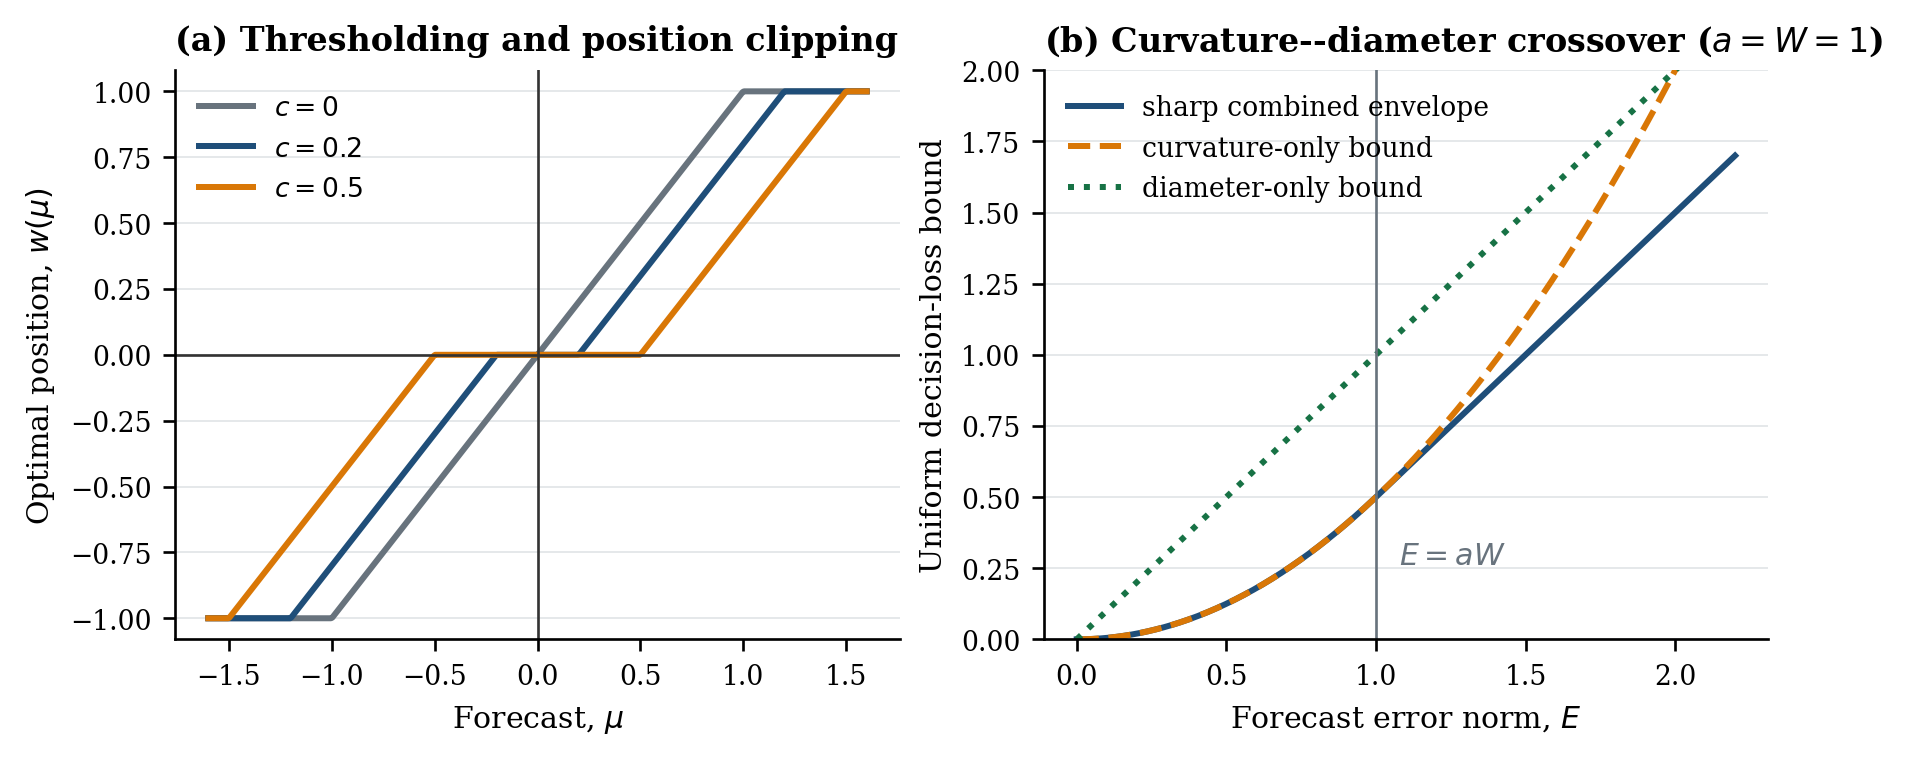
\includegraphics[width=\linewidth]{figures/01_decision_geometry.png}
\caption{Decision geometry under mixed frictions and constraints. Panel
(a) shows scalar soft thresholding with \(a=1\) and clipping to
\([-1,1]\) for three proportional-cost levels. Panel (b) compares the sharp
combined envelope \(C_{1,1}(E)\) in \eqref{eq:crossover} with the separate
curvature-only and diameter-only bounds. The combined inequality changes
branch at \(E=aW=1\), before the two separate bounds intersect.}
\label{fig:decisiongeometry}
\end{figure}

\subsection{Exact decisions from a forecast interval}
\label{sec:intervalposition}

A scalar certificate can sometimes retain the forecast interval
itself rather than replace it by a norm bound. For this subsection,
assume only that \(F:\R\to(-\infty,\infty]\) is proper, closed, and
convex. Let \(l<u\), and assume the conjugate values at both
endpoints are finite and attained. This includes the strongly
convex frictions above and purely proportional costs on a bounded
position set.

\begin{theorem}[The exact interval minimax position]
\label{thm:intervalposition}
For a fixed feasible position \(w\), the worst decision loss over
\(\mu\in[l,u]\) is
\begin{equation}\label{eq:intervalrisk}
 \mathcal R_{[l,u]}(w)
 :=\sup_{\mu\in[l,u]}\{F^*(\mu)-\mu w+F(w)\}
 =F(w)+\max\{F^*(l)-lw,F^*(u)-uw\}.
\end{equation}
An exact minimax position and its loss are
\begin{equation}\label{eq:secantposition}
 w_c=\frac{F^*(u)-F^*(l)}{u-l},\qquad
 \rho_{[l,u]}=F(w_c)+F^*(l)-lw_c .
\end{equation}
The position \(w_c\) is feasible. If \(F\) is strongly convex,
it is the unique minimax position. Integrable randomized positions
with well-defined expected losses cannot improve on this value.
\end{theorem}
\begin{proof}
For fixed \(w\), the expression being maximized is convex in
\(\mu\). Its maximum on the interval is therefore attained at
an endpoint, proving \eqref{eq:intervalrisk}.
Let \(w_l,w_u\) be conjugate maximizers at the two endpoints.
The two supporting-line inequalities for \(F^*\) give
\[
 w_l\le\frac{F^*(u)-F^*(l)}{u-l}\le w_u .
\]
Both endpoint maximizers belong to \(\operatorname{dom}F\);
convexity makes every point between them feasible, including
\(w_c\).

For \(w\le w_c\), the upper-endpoint term is the larger one, so
the risk is \(F(w)+F^*(u)-uw\). This convex function is
nonincreasing up to any of its minimizers \(w_u\ge w_c\).
For \(w\ge w_c\), the lower-endpoint term is larger and the
risk is nondecreasing beyond a minimizer \(w_l\le w_c\).
Consequently \(w_c\) minimizes the risk and equalizes the two
endpoint losses. Strong convexity of \(F\) makes the risk strongly
convex, giving uniqueness. Finally Jensen's inequality shows that
the mean of a randomized position has no larger expected loss
at any fixed \(\mu\); taking the worst case proves the last claim.
\end{proof}

For differentiable \(F^*\), this is a one-dimensional
convex-conjugate Bregman center. Chebyshev centers for Bregman
distances have an established general theory
\citep{BauschkeEtAl2010}. The scalar calculation above supplies
an explicit trading rule, also covering nonsmooth conjugates and
position bounds. Its uncertainty set is the whole interval.
If the interval is an outer enclosure of a constrained model
family, the minimax value for that smaller family can be lower.

\begin{corollary}[Quadratic and threshold minimax losses]
\label{cor:intervalradii}
For \(F(w)=aw^2/2\), \(a>0\), on \(\R\),
\[
 w_c=\frac{l+u}{2a},\qquad
 \rho_{[l,u]}=\frac{(u-l)^2}{8a}.
\]
For \(F(w)=c|w|+I_{[-1,1]}(w)\), \(c>0\), and
\([l,u]=[c-\epsilon,c+\epsilon]\) with \(0<\epsilon<c\),
\[
 w_c=\frac12,\qquad \rho_{[l,u]}=\frac{\epsilon}{2}.
\]
If \([l,u]\subseteq\partial F(w_0)\), then \(w_c=w_0\) and
\(\rho_{[l,u]}=0\).
\end{corollary}
\begin{proof}
The conjugates in the first two cases are
\(\mu^2/(2a)\) and \((|\mu|-c)_+\), respectively.
Substitution in \eqref{eq:secantposition} gives the formulas.
In the third case, conjugacy gives
\(F^*(\mu)=\mu w_0-F(w_0)\) throughout the interval.
\end{proof}

These are matching upper and lower bounds for the stated interval
information. In particular, the minimax loss is quadratic in
interval width under quadratic friction and linear at a purely
proportional trading threshold. The fractional threshold position
hedges uncertainty about the forecast. It solves a different
decision problem from maximizing profit at one fitted mean.


\section{Purely proportional costs and threshold decisions}

Now remove the quadratic term and impose \(|w|\le1\). Let
\[
V(w)=\E[\mu w-c|w|],\qquad c>0.
\]
Here \(c\) is the total proportional charge for the stipulated
one-period trade. The feasible bound and absence of quadratic curvature
distinguish this model from Section~2.

\begin{proposition}[Threshold rule and Gaussian value]\label{prop:threshold}
An optimal rule is
\[
w^\ast=\sgn(\mu)\mathbf1_{\{|\mu|>c\}},\qquad
V(w^\ast)=\E(|\mu|-c)_+.
\]
Ties at \(|\mu|=c\) are resolved by taking zero. If \(\mu\sim N(0,s^2)\),
\(s>0\), then, with \(\bar\Phi(z)=1-\Phi(z)\) the standard normal upper tail,
\begin{equation}\label{eq:gaussian}
V(w^\ast)=2\big[s\varphi(c/s)-c\,\bar\Phi(c/s)\big]
\sim2s\varphi(c/s)(s/c)^2,\qquad c/s\to\infty.
\end{equation}
\end{proposition}
\begin{proof}
On either half of the position interval the objective is linear, so
one of \(-1,0,1\) is optimal. The Gaussian formula follows by integrating
\(2\int_c^\infty(x-c)s^{-1}\varphi(x/s)\dd x\).
Using the Mills-ratio expansion
\(\bar\Phi(z)=\varphi(z)(z^{-1}-z^{-3}+O(z^{-5}))\)
gives the asymptotic expression.
\end{proof}

The Gaussian value is strictly positive for every \(s>0\).
At \(c/s=3\), it is approximately \(0.000764309\,s\);
the zero-cost value is \(s\sqrt{2/\pi}\). The retained fraction is
approximately \(0.09579\%\). This is a small positive oracle value,
not a claim that every weak predictor necessarily produces a loss.

\begin{theorem}[Exact threshold loss and its worst-case rate]\label{thm:thresholdloss}
Let
\(\widehat w=\sgn(\widehat\mu)\mathbf1_{\{|\widehat\mu|>c\}}\)
and \(\varepsilon=\widehat\mu-\mu\).
The pointwise regret is
\begin{align}
L={}&(|\mu|-c)\mathbf1_{\{w^\ast\ne0,\widehat w=0\}}
 +(c-\widehat w\mu)\mathbf1_{\{w^\ast=0,\widehat w\ne0\}}\notag\\
&+2|\mu|\mathbf1_{\{\widehat w=-w^\ast\ne0\}}.
\label{eq:thresholdloss}
\end{align}
It satisfies \(0\le L\le2|\varepsilon|\), so
\(\E L\le2\sqrt{\E\varepsilon^2}\).
There is no constant \(C\), independent of the joint law, such that
\(\E L\le C\E\varepsilon^2\) for every such problem.
\end{theorem}
\begin{proof}
Enumerate the cases where both decisions agree, where one is zero,
and where they have opposite nonzero signs to obtain
\eqref{eq:thresholdloss}. The optimality of \(\widehat w\) for
\(\widehat\mu\) gives
\[
L\le(\mu-\widehat\mu)(w^\ast-\widehat w)\le2|\varepsilon|.
\]
For the final assertion take \(0<h<c\), \(0<u<h\),
\(\mu=c+h\), and \(\widehat\mu=c-u\).
Then \(L=h\) while \(\varepsilon^2=(h+u)^2\).
Letting \(u\downarrow0\) and then \(h\downarrow0\) makes the ratio
unbounded.
\end{proof}

The counterexample concentrates mass \emph{near} a moving decision
boundary as the error shrinks. It is a worst-case obstruction, not a
universal first-order rate for a fixed smooth distribution. The
bound \(L\le2|\varepsilon|\) also shows that MSE consistency implies
decision consistency in this bounded-position model.

\begin{proposition}[A smooth-law expansion]\label{prop:smooth}
Suppose \(\mu\) has a density \(f\) continuous and bounded on
neighborhoods of \(c\) and \(-c\). Let a family of errors
\(\varepsilon_s\), independent of \(\mu\), satisfy
\(\E\varepsilon_s^2=s^2\to0\) and
\(\E|\varepsilon_s|^3=O(s^3)\). Then
\begin{equation}\label{eq:smooth}
\E L=\tfrac12[f(c)+f(-c)]s^2+o(s^2).
\end{equation}
Centering the errors is not required.
\end{proposition}
\begin{proof}
Choose \(d>0\) smaller than \(c\) and the radii of the density
neighborhoods. On \(\{|\varepsilon_s|\le d\}\), opposite nonzero
positions cannot occur. Conditional on an error \(e\), the contribution
from crossing \(+c\) is an integral of \(h f(c\pm h)\) over
\(0<h<|e|\), with the sign selected by the sign of \(e\).
Continuity makes this
\(\frac12 f(c)e^2+o(e^2)\), uniformly as \(e\to0\).
The same argument applies at \(-c\).
For larger errors,
\[
\E[L\mathbf1_{\{|\varepsilon_s|>d\}}]
\le2\E[|\varepsilon_s|\mathbf1_{\{|\varepsilon_s|>d\}}]
\le\frac{2}{d^2}\E|\varepsilon_s|^3=O(s^3).
\]
Likewise
\(\E[\varepsilon_s^2\mathbf1_{\{|\varepsilon_s|>d\}}]
\le d^{-1}\E|\varepsilon_s|^3=O(s^3)\).
Choosing a small fixed \(d\), then using uniform continuity on the
remaining neighborhood, establishes the averaged \(o(s^2)\) remainder.
\end{proof}

Under the independence assumptions and a fixed \(f\), the leading
coefficient is the same for all such small error families.
With errors correlated with the signal, the allocation of error near
the thresholds matters as well. A decision-focused loss can distinguish
forecasts with equal global MSE, but the threshold model does not
invalidate squared-error estimation of a conditional mean.

\subsection{Margin rates without independent errors}

The smooth expansion above uses independence. Without it, a small
global MSE can concentrate precisely where trading changes sign or
switches on. Let
\[
D=\big||\mu|-c\big|
\]
be distance to the nearest trading threshold. Assume a margin bound
\begin{equation}\label{eq:marginassumption}
\mathbb P(D\le z)\le C z^\alpha,\qquad 0<z\le z_0,
\quad C>0,\quad\alpha>0.
\end{equation}
It excludes mass exactly at the thresholds but allows arbitrary
dependence between \(\mu\) and its estimation error.

\begin{theorem}[Threshold rates under a margin condition]\label{thm:margin}
For the bounded-position proportional-cost decision and
\eqref{eq:marginassumption}, the following bounds hold.
If \(|\varepsilon|\le e\le z_0\) almost surely, then
\[
\E L\le2C e^{\alpha+1}.
\]
If only \(\E\varepsilon^2\le s^2\) is known, then for every
\(0<z\le z_0\),
\begin{equation}\label{eq:msemargin}
\E L\le2Cz^{\alpha+1}+\frac{2s^2}{z}.
\end{equation}
Consequently, for sufficiently small \(s\),
\(\E L=O((s^2)^{(\alpha+1)/(\alpha+2)})\).
For every \(\alpha>0\), this exponent cannot be increased uniformly
under only the stated MSE and margin assumptions, even with a fixed
law of \(\mu\).
\end{theorem}
\begin{proof}
Whenever the true and estimated decisions differ, the interval
between \(\mu\) and \(\widehat\mu\) crosses at least one threshold.
Thus \(D\le|\varepsilon|\) on the event of positive loss, and
Theorem~\ref{thm:thresholdloss} strengthens to
\[
L\le2|\varepsilon|\mathbf1_{\{D\le|\varepsilon|\}}.
\]
The uniform-error bound follows directly. Split the expectation
at \(|\varepsilon|=z\). On the lower part use
\(2z\mathbf1_{\{D\le z\}}\); on the upper part use
\(2|\varepsilon|\le2\varepsilon^2/z\). This proves
\eqref{eq:msemargin}. The choice
\(z=[s^2/(C(\alpha+1))]^{1/(\alpha+2)}\) gives the rate.

For sharpness, fix \(0<d_0<c\) and a random variable \(D\) with
\(\mathbb P(D\le d)=(d/d_0)^\alpha\) on \([0,d_0]\).
Set \(\mu=c+D\). For \(0<t<d_0\), define
\(\varepsilon_t=-2D\mathbf1_{\{D\le t\}}\).
The estimated position is zero when \(D\le t\) and agrees with
the true unit long position otherwise. Direct integration gives
\begin{equation}\label{eq:marginlower}
\E L_t=\frac{\alpha\,t^{\alpha+1}}
                   {(\alpha+1)d_0^\alpha},\qquad
\E\varepsilon_t^2=\frac{4\alpha\,t^{\alpha+2}}
                   {(\alpha+2)d_0^\alpha}.
\end{equation}
Eliminating \(t\) gives a positive constant times
\((\E\varepsilon_t^2)^{(\alpha+1)/(\alpha+2)}\).
The signal law is unchanged as \(t\downarrow0\), proving sharpness.
\end{proof}

For a bounded positive density near the thresholds, \(\alpha=1\)
is available. An almost-sure error \(e\) then gives \(O(e^2)\);
an MSE budget alone gives the weaker sharp rate
\(O((\mathrm{MSE})^{2/3})\). The independent small-error expansion
of Proposition~\ref{prop:smooth} gives \(O(\mathrm{MSE})\) because
it rules out the concentration mechanism in \eqref{eq:marginlower}.
These are distinct assumptions, not inconsistent rates.

Figure~\ref{fig:thresholdrates} separates the small Gaussian oracle value
from the sharp decision-loss rate under dependent forecast errors.

\begin{figure}[tbp]
\centering
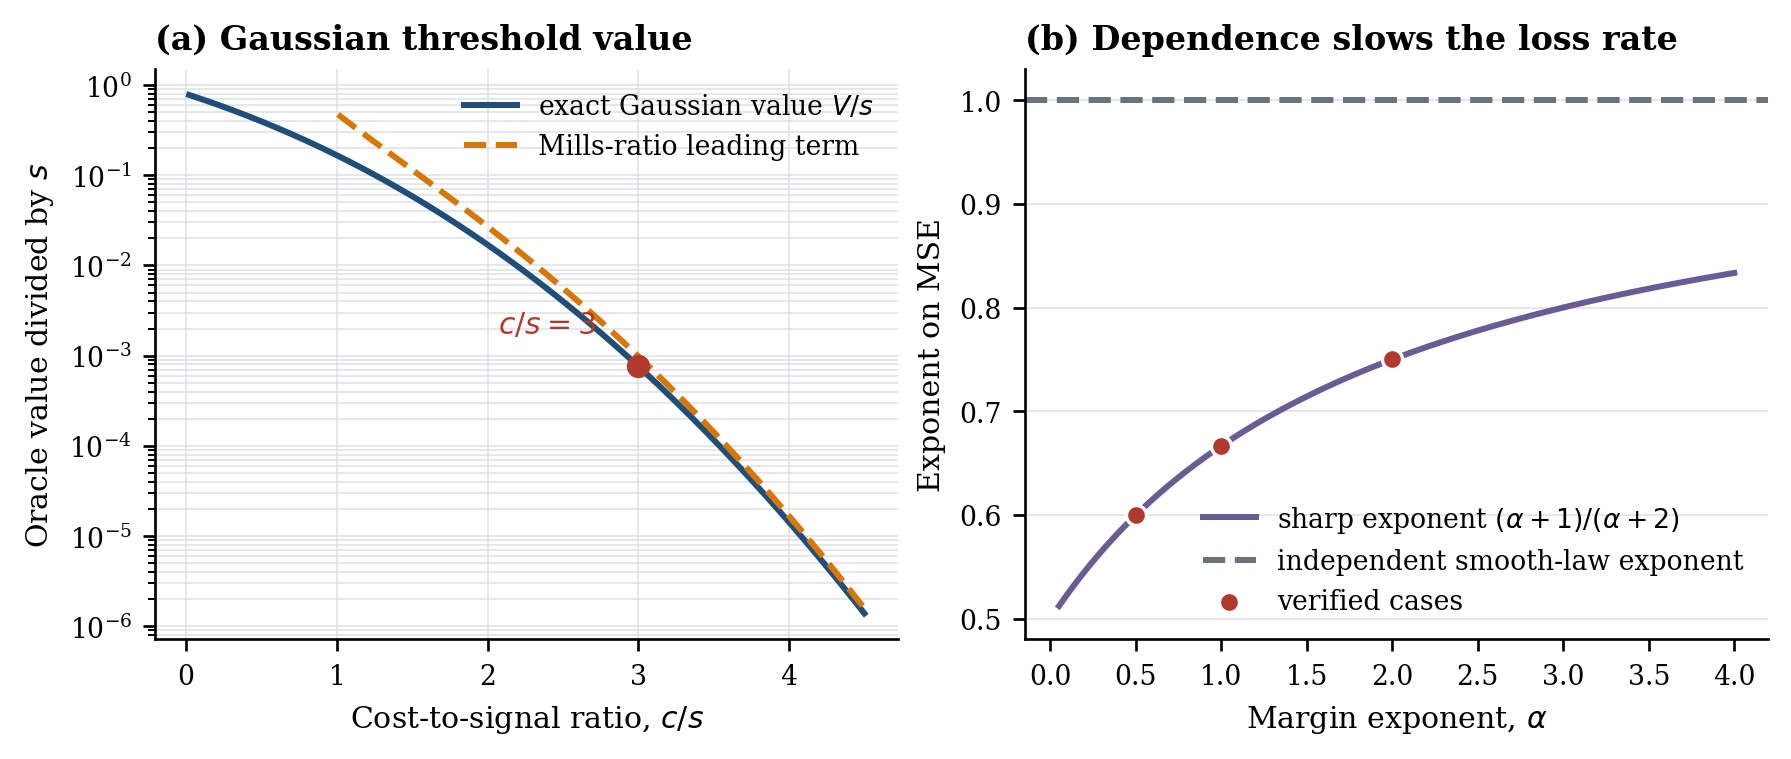
\includegraphics[width=\linewidth]{figures/02_threshold_rates.png}
\caption{Threshold value and threshold-loss rates. Panel (a) plots the
exact normalized Gaussian oracle value from \eqref{eq:gaussian} and its
Mills-ratio leading term; the marked point is \(c/s=3\). Panel (b) plots
the sharp exponent \((\alpha+1)/(\alpha+2)\) under only an MSE budget and
the margin condition, together with the verified fixed-law cases. The
dashed exponent one is the independent smooth-law benchmark of
Proposition~\ref{prop:smooth}; it relies on different assumptions.}
\label{fig:thresholdrates}
\end{figure}

\section{From order-book events and observations to a trading decision}

\subsection{Observable and hidden states}

Let \(X_t\) be a time-homogeneous Markov chain on a finite state space
\(\{1,\ldots,n\}\), with generator \(Q\), nonnegative off-diagonal
entries, and zero row sums. Its transition matrix is \(P_h=e^{hQ}\).
A bounded vector \(p\in\R^n\) assigns a reference price to each state.
The state may combine displayed queues, spread, recent flow, and a
latent liquidity regime. If a quantity is not observed, the trader
must use a posterior distribution rather than treat it as visible.
Write
\[
\pi_t(i)=\mathbb P(X_t=i\mid\mathcal G_t)
\]
for the row-vector posterior given pre-trade observations.
Assume the current reference price \(p_t=p(X_t)\) is observed and
that the model's Markov property holds for the full state.
The horizon-\(h\) conditional mean price change is then
\begin{equation}\label{eq:bookmean}
\mu_h(t)=\pi_t e^{hQ}p-p_t.
\end{equation}
The Markov property here includes the requirement that the observation
history contains no additional future information once \(X_t\) is given.

This is a local finite-state abstraction. A bounded price grid requires
an explicit boundary convention. For real books, time-of-day effects,
unmodeled order attributes, and hidden liquidity can invalidate the
state reduction. The estimates below are conditional on a specified
model and quantify perturbation within that model.

\subsection{A generator-to-regret certificate}

\begin{theorem}[Order-book model error transfer]\label{thm:booktransfer}
Let \(\widehat Q\) also be a valid generator on the same state space,
and let \(\widehat\pi_t\) be a probability vector. Use the same observed
current price and price vector to form
\(\widehat\mu_h(t)=\widehat\pi_t e^{h\widehat Q}p-p_t\).
Set
\[
\delta_Q=\norm{\widehat Q-Q}_{\infty\to\infty}
=\max_i\sum_j|\widehat Q_{ij}-Q_{ij}|,\qquad
B_p=\tfrac12(\max_i p_i-\min_i p_i).
\]
Then
\begin{equation}\label{eq:bookforecastbound}
|\widehat\mu_h(t)-\mu_h(t)|
\le B_p\big(\norm{\widehat\pi_t-\pi_t}_1+h\delta_Q\big).
\end{equation}
For an \(a\)-strongly convex trading friction,
\begin{equation}\label{eq:bookregret}
\mathcal L_F(\mu_h,\widehat\mu_h)
\le\frac{B_p^2}{2a}
\big(\norm{\widehat\pi_t-\pi_t}_1+h\delta_Q\big)^2.
\end{equation}
\end{theorem}
\begin{proof}
Stochastic matrices contract the sup norm. Duhamel's formula gives
\[
e^{h\widehat Q}-e^{hQ}
=\int_0^h e^{s\widehat Q}(\widehat Q-Q)e^{(h-s)Q}\dd s,
\]
hence the operator norm of this difference is at most \(h\delta_Q\).
Replace \(p\) by
\(p-\frac12(\max p+\min p)\mathbf1\), whose sup norm is \(B_p\).
Constants are annihilated by the difference of probability vectors
and by the difference of stochastic matrices. Splitting
\[
\widehat\pi_t e^{h\widehat Q}-\pi_t e^{hQ}
=(\widehat\pi_t-\pi_t)e^{hQ}
 +\widehat\pi_t(e^{h\widehat Q}-e^{hQ})
\]
proves \eqref{eq:bookforecastbound}. Apply
Theorem~\ref{thm:conjugate} to obtain \eqref{eq:bookregret}.
\end{proof}

\begin{corollary}[Estimation rates and the curvature boundary]
For fixed horizon, grid, and positive curvature modulus, if the
posterior error and generator error are both \(O_p(n_{\mathrm{obs}}^{-1/2})\),
the regret bound is \(O_p(n_{\mathrm{obs}}^{-1})\).
Under the purely proportional bounded-position model,
Theorem~\ref{thm:thresholdloss} instead gives the general bound
\[
L\le2B_p(\norm{\widehat\pi_t-\pi_t}_1+h\delta_Q).
\]
A faster rate there needs additional assumptions about the probability
mass and estimation errors near the trading thresholds.
\end{corollary}

The posterior error includes inference about latent liquidity.
An observed queue vector cannot be silently substituted for the
full state when hidden variables affect transitions.
The theorem does not provide a posterior estimator or establish
identifiability. A fitted matrix with negative off-diagonal entries is
not a generator and must be repaired before the contraction argument
can be used.

\begin{example}[Two-state calculation]\label{ex:twostate}
Let \(p=(0,1)^\top\) and
\[
Q=\begin{pmatrix}-\lambda&\lambda\\\lambda&-\lambda\end{pmatrix}.
\]
If state zero is observed, then \(\mu_h=(1-e^{-2\lambda h})/2\).
For \(h=1,\lambda=0.4,\widehat\lambda=0.6\), the true and estimated
means are approximately \(0.275336\) and \(0.349403\).
Here \(B_p=1/2\), \(\delta_Q=0.4\), and the forecast bound is \(0.2\),
compared with actual error approximately \(0.074067\).
With quadratic curvature \(a=2\), the exact decision loss is
approximately \(0.00137149\), below the certified upper bound \(0.01\).
All prices and costs in this example are synthetic model units.
\end{example}

\subsection{Relative-book states, price marks, and clock time}

A finite relative-book state need not confine the reference price to
a bounded grid. Let \(Z_t\) describe spread, relative queue depths, and
a possible hidden regime. At state \(z\), event channel \(e\) has rate
\(\lambda_e(z)\), next state \(T_e(z)\), and conditional mean price
increment \(\overline j_e(z)\). Price increments may occur even when
the relative state is unchanged. With between-event price drift
\(b_0(z)\), define
\begin{equation}\label{eq:markedbookgenerator}
 (Qu)_z=\sum_e\lambda_e(z)[u_{T_e(z)}-u_z],\qquad
 d_z=b_0(z)+\sum_e\lambda_e(z)\overline j_e(z).
\end{equation}
Assume finitely many states and channels, bounded rates and conditional
second moments of marks, and an integrable martingale component of the
price. Then compensation and the Markov property give
\begin{equation}\label{eq:additiveforecast}
 \mu_h(t)=\E[P_{t+h}-P_t\mid\mathcal G_t]
 =\pi_t\int_0^h e^{sQ}d\dd s.
\end{equation}
Indeed, the compensated price change has conditional mean zero, and
\(\E[d(Z_{t+s})\mid\mathcal G_t]=\pi_t e^{sQ}d\).
The vector \(d\) is the total price compensator. In the earlier bounded
price-vector model, \(d=Qp\), so integrating the semigroup derivative
recovers \eqref{eq:bookmean} when \(\pi_t p=p_t\).

Order-book event models of this type build on established Markov and
queue-reactive constructions
\citep{ContStoikovTalreja2010,HuangLehalleRosenbaum2015}.
The distinction between a relative state and an additive price is
essential to their use in a forecast certificate. The generator of the
relative state alone does not specify the price marks or the event clock.

\begin{example}[The clock and the marks cannot be discarded]
\label{ex:bookclock}
Consider a single relative state, with unit upward price events of
rate \(\lambda p\) and downward events of rate \(\lambda(1-p)\).
The relative-state generator is \(Q=0\), but
\(\mu_h=h\lambda(2p-1)\). For \(p=3/4\) and \(h=1\), rates
\(\lambda=1\) and \(\lambda=4\) give means \(1/2\) and \(2\).
The relative-state generator and the upward probability per event
are identical in the two models. Neither object alone determines a
clock-time price forecast.
\end{example}

For a vector \(u\), write
\(\spn(u)=\max_i u_i-\min_i u_i\). A stochastic semigroup always
contracts span. When a stronger bound
\begin{equation}\label{eq:spanmixing}
 \spn(e^{sQ}u)\le e^{-\omega s}\spn(u),\qquad s\ge0,
\end{equation}
is available for some \(\omega>0\), it improves the horizon dependence.
We allow \(\omega=0\), which requires no mixing assumption, and set
\begin{align}
 A_\omega(h)&=\int_0^h e^{-\omega s}\dd s
 =\begin{cases}(1-e^{-\omega h})/\omega,&\omega>0,\\h,&\omega=0,
 \end{cases}\label{eq:mixA}\\
 C_\omega(h)&=\int_0^h A_\omega(s)\dd s
 =\begin{cases}h/\omega-(1-e^{-\omega h})/\omega^2,&\omega>0,\\
 h^2/2,&\omega=0.
 \end{cases}\label{eq:mixC}
\end{align}

\begin{proposition}[Forecast transfer for an additive price]
\label{prop:additivetransfer}
Let \(Q,\widehat Q\) be valid generators, \(\pi,\widehat\pi\)
probability rows, and \(d,\widehat d\) price-compensator vectors on the
same finite state space. Suppose \(Q\) satisfies
\eqref{eq:spanmixing}. With
\[
 D_d=\tfrac12\spn(d),\quad
 \delta_\pi=\norm{\pi-\widehat\pi}_1,\quad
 \delta_Q=\norm{Q-\widehat Q}_{\infty\to\infty},\quad
 \varepsilon_d=\norm{d-\widehat d}_\infty,
\]
the forecasts defined by \eqref{eq:additiveforecast} satisfy
\begin{equation}\label{eq:additivebound}
 |\mu_h-\widehat\mu_h|
 \le h\varepsilon_d+
 D_d\{A_\omega(h)\delta_\pi+C_\omega(h)\delta_Q\}.
\end{equation}
\end{proposition}
\begin{proof}
The posterior term at time \(s\) is bounded by
\(D_d e^{-\omega s}\delta_\pi\), because a zero-sum row annihilates
constants and can be applied to the centered vector \(e^{sQ}d\).
For the generator term, use
\[
 (e^{s\widehat Q}-e^{sQ})d
 =\int_0^s e^{(s-v)\widehat Q}
            (\widehat Q-Q)e^{vQ}d\dd v.
\]
The left semigroup contracts the sup norm, the rate difference
annihilates constants, and \eqref{eq:spanmixing} bounds the centered
right vector by \(D_d e^{-\omega v}\). Thus this term is at most
\(D_d\delta_Q A_\omega(s)\). The drift-vector error is at most
\(\varepsilon_d\) at every time under the estimated semigroup.
Integrating the three bounds proves \eqref{eq:additivebound}.
\end{proof}

Applying Theorem~\ref{thm:conjugate} squares this forecast bound and
divides by \(2a\). A bounded position domain allows the sharper
envelope \(C_{a,W}\) of Proposition~\ref{prop:crossover}.
A positive \(\omega\) is an additional verified property, not a
consequence of merely having a finite generator. It changes the
generator contribution from quadratic to asymptotically linear in
\(h\); a constant compensator error still accumulates linearly.

\begin{proposition}[Sharp horizon and mixing coefficients]
\label{prop:sharpbookconstants}
Each of the three coefficients \(h,A_\omega(h),C_\omega(h)\)
in \eqref{eq:additivebound} is individually best possible over
the stated class. The generator coefficient is approached by
two-state marked-event models.
\end{proposition}
\begin{proof}
Fix \(D>0,\omega\ge0,h>0\), and use
\[
 Q_0=\begin{pmatrix}0&0\\ \omega&-\omega\end{pmatrix},
 \qquad d=\binom0D,\qquad \pi=(1,0).
\]
Its span contraction is exactly \(e^{-\omega s}\).
Changing only the posterior to \((1-\eta,\eta)\), with
\(0\le\eta\le1\), changes the forecast by
\(D\eta A_\omega(h)\). Since \(D_d=D/2\) and
\(\delta_\pi=2\eta\), this attains the posterior term.
Changing only the compensator to \(d+c\mathbf1\) changes the
forecast by \(hc\), attaining the drift term in absolute value.

Now leave \(d,\pi\) unchanged and set
\[
 Q_\epsilon=
 \begin{pmatrix}-\epsilon&\epsilon\\
                  \omega&-\omega\end{pmatrix},\qquad \epsilon>0.
\]
The baseline forecast is zero, while the perturbed forecast is
\[
 D\int_0^h\frac{\epsilon}{\omega+\epsilon}
                      (1-e^{-(\omega+\epsilon)s})\dd s
 =D\epsilon C_{\omega+\epsilon}(h).
\]
Here \(\delta_Q=2\epsilon\), so the ratio of actual error to
the generator term \(D\epsilon C_\omega(h)\) tends to one as
\(\epsilon\downarrow0\). This also covers \(\omega=0\).
Both models have a marked-event realization: the states describe
two liquidity regimes, their transitions carry no price mark,
and unit upward price events occur at rate \(D\) in the second
state without changing that state.
\end{proof}

With \(\omega=0\), the last construction has forecast error
\(D\epsilon h^2/2+O(\epsilon^2)\) for fixed \(h\).
Under unconstrained quadratic friction its decision loss is
\(D^2\epsilon^2h^4/(8a)+O(\epsilon^3)\).
Thus the fourth power of the horizon in this nonmixing
generator-to-loss bound is attainable locally; it is not solely
an artifact of applying two inequalities.


\subsection{Filtering hidden states from events and quiet periods}

The preceding results require a posterior. We now specify a finite
event-observation model and give a pathwise error allowance for that
posterior. Let \(U\) be the generator of unobserved state transitions.
For each observed event type \(e\), let \(M_e\) be a nonnegative matrix:
\(M_e(i,j)\) is the rate of an event of type \(e\) that also changes
the state from \(i\) to \(j\). Diagonal entries are permitted, because
an observed event can leave the hidden state unchanged. Define
\begin{equation}\label{eq:eventfiltermatrices}
 \nu=\sum_e M_e\mathbf1,\qquad
 K=U-\operatorname{diag}(\nu),\qquad
 Q=K+\sum_e M_e.
\end{equation}
Then \(K\) is a subgenerator for evolution without an observed event,
and \(Q\) is the generator of the full latent state. These
point-process filtering principles are classical; see
\citet{Snyder1972}. The formulas here retain simultaneous event and
state changes, as an order-book observation can require.

\begin{proposition}[Event-history posterior and its perturbation]
\label{prop:eventfilter}
Starting with prior \(\pi_0\), suppose the observed history by time
\(t\) consists of events \(e_1,\ldots,e_N\) at ordered times, with
successive waiting intervals \(\Delta_1,\ldots,\Delta_{N+1}\) summing
to \(t\). The posterior is the normalized row
\begin{equation}\label{eq:exacteventfilter}
 \alpha=\pi_0e^{K\Delta_1}M_{e_1}e^{K\Delta_2}
                 \cdots M_{e_N}e^{K\Delta_{N+1}},\qquad
 \pi_t=\frac{\alpha}{\alpha\mathbf1},
\end{equation}
provided its denominator is positive. This denominator is a history
density with respect to event times and types, not the probability of
an exact continuous-time history.

For two valid models, choose common constants \(a_e>0\) at least as
large as every row sum of both \(M_e\) and \(\widehat M_e\), and put
\(B_e=M_e/a_e\), \(\widehat B_e=\widehat M_e/a_e\).
Let \(L\) be the product in \eqref{eq:exacteventfilter} with
\(B_e\) in place of \(M_e\), and let \(\widehat L\) be its fitted
counterpart. Define the rescaled likelihoods
\[
 Z=\pi_0L\mathbf1,\qquad
 \widehat Z=\widehat\pi_0\widehat L\mathbf1
\]
and the supplied bounds
\begin{align*}
 \norm{\pi_0-\widehat\pi_0}_1&\le\varepsilon_0,&
 \norm{K-\widehat K}_{\infty\to\infty}&\le\varepsilon_K,&
 \norm{B_e-\widehat B_e}_{\infty\to\infty}&\le\varepsilon_{B,e}.
\end{align*}
If \(Z,\widehat Z>0\), then
\begin{equation}\label{eq:filtererror}
 \norm{\pi_t-\widehat\pi_t}_1
 \le\varepsilon_\pi(t):=
 \min\left\{2,\frac{2}{\widehat Z}
       \left(\varepsilon_0+t\varepsilon_K+
             \sum_{k=1}^N\varepsilon_{B,e_k}\right)\right\}.
\end{equation}
\end{proposition}
\begin{proof}
Before an observed event, unnormalized conditional mass evolves by
\(\dot\alpha=\alpha K\); survival requires accounting for the
state-dependent observed-event hazard. At an event of type \(e\),
its likelihood and any simultaneous state transition multiply that
row by \(M_e\). Iteration proves \eqref{eq:exacteventfilter}.
Dividing each event matrix by a common positive scalar changes the
unnormalized row by a scalar and leaves its normalization unchanged.

The matrices \(B_e,e^{K\Delta}\), and their fitted versions are
substochastic. They contract row \(\ell^1\) norms, and their induced
sup norms are at most one. Duhamel's formula gives
\(\norm{e^{K\Delta}-e^{\widehat K\Delta}}_{\infty\to\infty}
\le\Delta\varepsilon_K\). Telescoping the product therefore yields
\[
 \norm{\pi_0L-\widehat\pi_0\widehat L}_1
 \le E_{\rm hist}:=\varepsilon_0+t\varepsilon_K+
                      \sum_{k=1}^N\varepsilon_{B,e_k}.
\]
In particular \(|Z-\widehat Z|\le E_{\rm hist}\). With
\(u=\pi_0L\) and \(\widehat u=\widehat\pi_0\widehat L\),
\[
 \norm{u/Z-\widehat u/\widehat Z}_1
 \le\frac{|\widehat Z-Z|+\norm{u-\widehat u}_1}{\widehat Z}
 \le\frac{2E_{\rm hist}}{\widehat Z}.
\]
Two probability vectors are at most two apart, giving the minimum.
\end{proof}

The common scaling constants make the product bound explicit; they
do not turn the rescaled likelihood into a probability of the exact
history. Rare histories can make the bound uninformative. If
\(\widehat Z=0\), the fitted posterior is undefined, so an additional
support or regularization convention is needed. No uniform filtering
stability or hidden-regime identifiability is asserted without
additional assumptions. Observed price changes and other marks used
by the trader must be included in the observation history. Known past
actions can be conditioned on in a controlled event model, but the
future forecasts here use the declared exogenous law.

\begin{example}[Silence is an observation]\label{ex:silence}
There are two fixed hidden regimes, fast and slow, with observed
event rates \(3\) and \(1\) and equal prior probabilities. Here
\(U=0\), \(M=\operatorname{diag}(3,1)\), and
\(K=-\operatorname{diag}(3,1)\). No event for one unit of time gives
\[
 \mathbb P(\text{fast}\mid\text{no event by }1)
 =\frac{e^{-3}}{e^{-3}+e^{-1}}
 =\frac1{1+e^2}\approx0.119203.
\]
In contrast, an event observed with negligible waiting time from the
equal prior gives fast-regime probability \(3/4\). If each event
carries a unit upward price mark, the expected price increase over
the next unit of time after the quiet period is approximately
\(1.238406\), compared with the unconditional value \(2\).
This synthetic example isolates the information in waiting times;
it is not a calibrated price model.
\end{example}

\subsection{State reduction and a complete decision certificate}

Queue features are often compressed before forecasting. Equality of
displayed depth does not ensure equality of future event laws: two
tagged orders can have different quantities ahead, and a hidden regime
can change event rates without changing the snapshot. We quantify
the effect of a specified finite state reduction.

Let \(c:\{1,\ldots,n\}\to\{1,\ldots,m\}\) be a surjective cell map
and let \(L_{i\ell}=\mathbf1_{\{c(i)=\ell\}}\) lift a coarse vector
to the full state space. In this subsection \(L\) denotes this lift,
not the likelihood product in Proposition~\ref{prop:eventfilter}.
For a valid coarse generator \(\overline Q\), put
\begin{equation}\label{eq:lumpresidual}
 R=QL-L\overline Q,\qquad
 \delta_R=\norm{R}_{\infty\to\infty}.
\end{equation}
The following intertwining criterion is the finite-chain strong
lumpability criterion \citep{Buchholz1994}; it is included to make
the state-reduction assumption checkable.

\begin{proposition}[Exact and approximate state reduction]
\label{prop:aggregation}
The identity \(e^{sQ}L=Le^{s\overline Q}\) for every \(s\ge0\)
holds if and only if \(R=0\). Equivalently, for every full state
\(i\) and coarse cell \(b\),
\begin{equation}\label{eq:cellrates}
 \sum_{j:c(j)=b}Q_{ij}=\overline Q_{c(i),b}.
\end{equation}
In general,
\begin{equation}\label{eq:intertwiningerror}
 e^{sQ}L-Le^{s\overline Q}
 =\int_0^s e^{(s-v)Q}R e^{v\overline Q}\dd v.
\end{equation}
\end{proposition}
\begin{proof}
Differentiate the exact identity at zero to obtain \(R=0\).
Conversely, \(QL=L\overline Q\) implies
\(Q^kL=L\overline Q^k\) for every integer \(k\ge0\), hence the
semigroup identity by its power series. Matrix multiplication gives
\eqref{eq:cellrates}. Differentiating
\(e^{(s-v)Q}Le^{v\overline Q}\) in \(v\) and integrating proves
\eqref{eq:intertwiningerror}.
\end{proof}

Thus aggregate rates to every coarse cell must agree within each
cell of the full state space. Even when this condition holds, a
coarse price forecast also requires compatibility of the price
compensator; state-transition lumpability alone omits marked events
that leave the state unchanged.

\begin{corollary}[When filtering can also be reduced]
\label{cor:filterreduction}
In the event-observation model of Proposition~\ref{prop:eventfilter},
suppose a valid coarse observation model satisfies
\[
 KL=L\overline K,\qquad M_eL=L\overline M_e
 \quad\text{for every observed type }e.
\]
Starting from coarse prior \(\pi_0L\), its event-history posterior
equals \(\pi_tL\) whenever the history has positive likelihood.
\end{corollary}
\begin{proof}
The first equality implies \(e^{sK}L=Le^{s\overline K}\).
Successively commuting the lift through the event-history product
gives \(\alpha L=\overline\alpha\). Since
\(L\mathbf1=\mathbf1\), the two likelihood normalizers agree.
Normalizing therefore gives the claimed posterior identity.
\end{proof}

The forecast reduction below does not by itself authorize running
the filter on a compressed state. It uses a supplied full-state
posterior, which may then be aggregated. The additional conditions in
Corollary~\ref{cor:filterreduction} give one exact way to reduce the
filter too. Lumpability of \(Q=K+\sum_eM_e\) alone does not impose
the separate equalities for survival and each observed event type.

\begin{theorem}[From event observations to position loss]
\label{thm:bookdecision}
Let \(\pi_t,Q,d\) describe the full conditional forecast
\eqref{eq:additiveforecast}. Let \(\widehat\pi_t\) be a fitted
posterior and \((\overline Q,\overline d)\) a coarse forecast model,
with deployed forecast
\begin{equation}\label{eq:coarseforecast}
 \widehat\mu_h=(\widehat\pi_t L)
                 \int_0^h e^{s\overline Q}\overline d\dd s.
\end{equation}
Suppose the coarse semigroup satisfies the span contraction
\eqref{eq:spanmixing} with \(\overline Q\) in place of \(Q\).
Set \(\overline D=\spn(\overline d)/2\) and assume
\[
 \norm{\pi_t-\widehat\pi_t}_1\le\varepsilon_\pi,\qquad
 \norm{d-L\overline d}_\infty\le\delta_d,\qquad
 \norm{QL-L\overline Q}_{\infty\to\infty}\le\delta_R.
\]
Then
\begin{equation}\label{eq:completebookerror}
 |\mu_h-\widehat\mu_h|\le
 E_h:=h\delta_d+\overline D\{
       A_\omega(h)\varepsilon_\pi+C_\omega(h)\delta_R\}.
\end{equation}
In particular, \(\varepsilon_\pi\) may be supplied by
\eqref{eq:filtererror}. If a fitted full model satisfies
\(\norm{Q-\widehat Q}_{\infty\to\infty}\le\varepsilon_Q\)
and \(\norm{d-\widehat d}_\infty\le\varepsilon_d\), valid
computable choices are
\begin{equation}\label{eq:computedreduction}
 \delta_R=\norm{\widehat QL-L\overline Q}_{\infty\to\infty}
               +\varepsilon_Q,\qquad
 \delta_d=\norm{\widehat d-L\overline d}_\infty+\varepsilon_d.
\end{equation}

Let \(F\) be the known proper closed \(a\)-strongly convex trading
friction, including its convex constraints, and assume the true
optimizer \(w^*\) exists. For an implemented feasible position
\(\widetilde w\), suppose a subgradient
\(g\in\partial F(\widetilde w)\) is available and
\(|g-\widehat\mu_h|\le\chi\). If the effective domain of \(F\)
has diameter at most \(W\), the actual objective loss satisfies
\begin{equation}\label{eq:completebookloss}
 [\mu_h w^*-F(w^*)]-
 [\mu_h\widetilde w-F(\widetilde w)]
 \le C_{a,W}(E_h+\chi).
\end{equation}
On an unbounded domain the right side can be replaced by
\((E_h+\chi)^2/(2a)\). An exact fitted optimizer has \(\chi=0\).
\end{theorem}
\begin{proof}
First replace \(d\) by \(L\overline d\) inside the true forecast;
sup-norm contraction bounds the resulting error by \(h\delta_d\).
Next use \eqref{eq:intertwiningerror}. The rows of \(R\) sum to zero,
so \(R\) annihilates constants. Coarse span contraction bounds the
centered vector \(e^{v\overline Q}\overline d\) by
\(\overline D e^{-\omega v}\), while the full semigroup contracts
the sup norm. Integrating over \(v\), then over the forecast horizon,
gives \(\overline D C_\omega(h)\delta_R\).
The remaining posterior difference has zero total mass and is
bounded by \(\overline D A_\omega(h)\varepsilon_\pi\).
This proves \eqref{eq:completebookerror}. Since
\(\norm{L}_{\infty\to\infty}=1\), the triangle inequality gives
\eqref{eq:computedreduction}.

For the final step, strong convexity at \(\widetilde w\) gives,
with \(v=w^*-\widetilde w\),
\[
 [\mu_hw^*-F(w^*)]-[\mu_h\widetilde w-F(\widetilde w)]
 \le(\mu_h-g)v-\tfrac a2 v^2
 \le(E_h+\chi)|v|-\tfrac a2|v|^2.
\]
Maximizing over \(0\le|v|\le W\) yields
\(C_{a,W}(E_h+\chi)\); maximizing over \(|v|\ge0\) yields the
unbounded-domain bound. At an exact fitted optimum,
\(\widehat\mu_h\in\partial F(\widetilde w)\), so \(\chi=0\).
\end{proof}

The certificate keeps event-history inference, model uncertainty,
state reduction, price marks, and optimizer accuracy as distinct
quantities. It is conditional on valid event and generator models and
supplied parameter-error bounds. The filtering formula does not
estimate those bounds from data, and a small in-sample forecast error
does not certify them. If trading materially changes the future book
law, that effect must be modeled in the control problem. Here the
book forecast is exogenous to the chosen position, and known trading
costs enter \(F\); Section~6 treats error in an impact operator on a
specified common probability space.

\begin{example}[An event-history certificate in trading units]
\label{ex:completebook}
Consider four hidden liquidity states, reduced to cells
\(\{1,2\}\) and \(\{3,4\}\). Let
\[
 Q_0=\begin{pmatrix}
 -1.6&1&0.4&0.2\\
 0.3&-0.9&0.1&0.5\\
 0.2&0.2&-1.1&0.7\\
 0.3&0.1&0.8&-1.2
 \end{pmatrix},
 \qquad E_{24}=1,\quad E_{22}=-1,
\]
with all other entries of \(E\) zero. The unobserved generators are
\(U=Q_0+0.02E\) and \(\widehat U=Q_0+0.023E\).
Observed events have unit price marks \(+1\) and \(-1\), with
\[
 M_+=\operatorname{diag}(1.5,1.56,0.5,0.52),\qquad
 M_-=\operatorname{diag}(0.65,0.66,1.2,1.22).
\]
Set \(\widehat M_+=1.001M_+\) and
\(\widehat M_-=0.999M_-\). Because these observed events leave the
hidden state unchanged, \(Q=U\) and \(\widehat Q=\widehat U\),
while \(d=(M_+-M_-)\mathbf1\) and
\(\widehat d=(\widehat M_+-\widehat M_-)\mathbf1\).

The true and fitted priors are \((0.4,0.1,0.3,0.2)\) and
\((0.401,0.099,0.3,0.2)\). Observe events \(+,-,+\) with waiting
intervals \(0.08,0.11,0.04\), followed by a quiet interval \(0.09\).
Use the smallest common row-sum upper bounds as the constants
\(a_e\) in Proposition~\ref{prop:eventfilter}. If \(L\) is the cell
lift, set \(A=L^\top/2\),
\(\overline Q=A\widehat QL\), and
\(\overline d=A\widehat d\). The coarse two-state contraction rate
is \(\omega=\overline Q_{12}+\overline Q_{21}=1.0115\).

For horizon \(h=0.7\), curvature \(a=0.7\), starting position
\(w_0=0.04\), and friction
\[
 F(w)=0.35w^2+0.02|w-0.04|+I_{[-0.6,0.6]}(w),
\]
deploy the exact coarse-forecast optimizer plus a position error of
\(0.007\). This position is interior, and its subgradient residual
is \(\chi=0.0049\). Direct matrix exponentials and convex optimization
give the following quantities, rounded for display:
\begin{center}
\begin{tabular}{@{}lr@{}}
\toprule
Quantity&Value\\
\midrule
Rescaled fitted history likelihood \(\widehat Z\)&0.15267510\\
Posterior error allowance \(\varepsilon_\pi\)&0.09439656\\
Rate-reduction allowance \(\delta_R\)&0.02900000\\
Price-compensator allowance \(\delta_d\)&0.02725500\\
True forecast \(\mu_h\)&0.21587418\\
Deployed forecast \(\widehat\mu_h\)&0.21629237\\
Forecast error allowance \(E_h\)&0.06085928\\
Actual decision loss&0.00002020\\
Certified decision loss \(C_{a,1.2}(E_h+\chi)\)&0.00308877\\
\bottomrule
\end{tabular}
\end{center}
The bound uses uniform parameter enclosures and a pathwise filtering
allowance, so it need not be attained in this example.
All rates, priors, costs, and marks in this example are
synthetic, and the uncertainty allowances are computed from its two
specified models. The example checks a conditional certificate, not a
statistical confidence set learned from market data.
\end{example}

Figure~\ref{fig:filtercertificate} visualizes the two stages that are easy
to conflate: history filtering and downstream loss certification.

\begin{figure}[tbp]
\centering
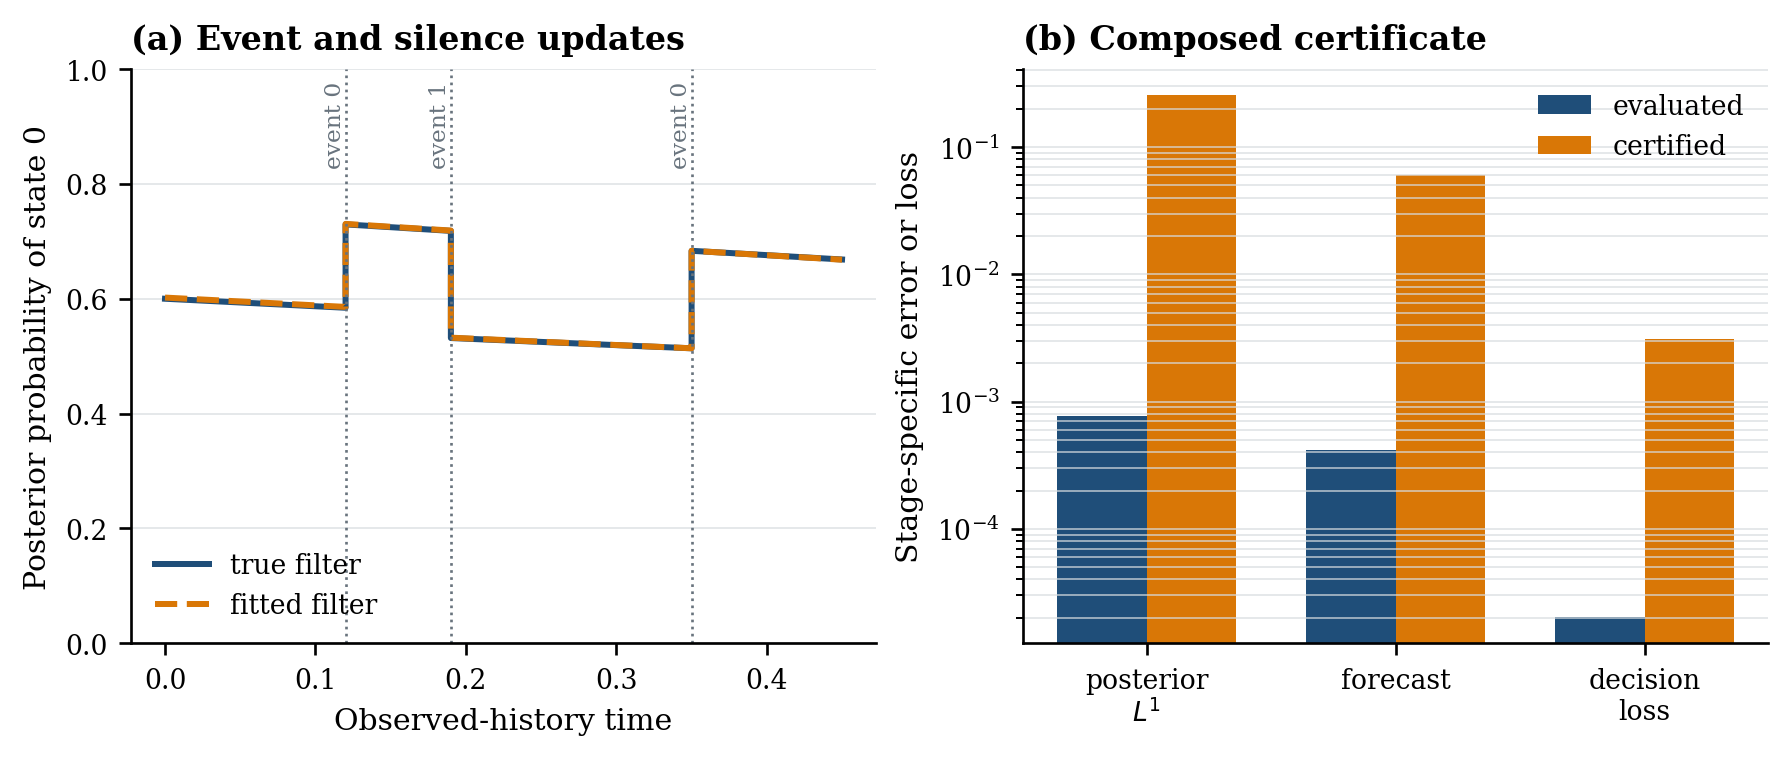
\includegraphics[width=\linewidth]{figures/03_filter_certificate.png}
\caption{Event filtering and a composed decision certificate in two
complementary synthetic cells. Panel (a) shows true and fitted two-state
posteriors along a fixed observed history: events cause likelihood jumps,
while each quiet interval evolves the posterior continuously. Panel (b)
compares the independently evaluated posterior error, forecast error, and
decision loss with their corresponding allowances in the verified
event-to-position calculation. The stages have different units and are
compared only within each pair; no market data or fitted confidence level
is asserted.}
\label{fig:filtercertificate}
\end{figure}

\subsection{State reduction specific to the price forecast}
\label{sec:pricesufficient}

Preserving every transition probability is stronger than preserving
the conditional mean used by a particular trading objective.
Let \(L\) lift functions on a partition into vectors constant on
each cell, as above. Write
\[
 v_h=\int_0^h e^{sQ}d\dd s.
\]
The feature preserves the horizon-\(h\) conditional mean exactly
when \(v_h\in\operatorname{im}L\). This criterion concerns the
specified additive price compensator and the known, common
friction \(F\). It does not assert that conditional variances,
fill probabilities, or inventory-dependent rewards are preserved.

\begin{proposition}[A finite test for price-mean sufficiency]
\label{prop:pricekrylov}
For a generator on \(n\) states, the following are equivalent:
\[
 v_h\in\operatorname{im}L\quad\hbox{for every }h\ge0;
 \qquad
 Q^j d\in\operatorname{im}L,\quad j=0,\ldots,n-1.
\]
Thus the feature need only preserve the subspace generated by
\(d,Qd,\ldots,Q^{n-1}d\), rather than all vectors constant on
its cells. Full transition lumpability implies this condition
when \(d\in\operatorname{im}L\), but the converse can fail.
\end{proposition}
\begin{proof}
The map \(h\mapsto v_h\) is analytic, with
\(v_h=\sum_{j\ge0}h^{j+1}Q^jd/(j+1)!\).
If \(v_h\) belongs to the closed linear subspace
\(\operatorname{im}L\) for every \(h\ge0\), all its right
derivatives at zero do too. These derivatives give every \(Q^jd\).
Conversely, the Cayley--Hamilton identity expresses all powers
of \(Q\) of order at least \(n\) as combinations of its first
\(n\) powers. The finite condition therefore places every term
of the convergent series in \(\operatorname{im}L\).
Under full lumpability, that image is \(Q\)-invariant, giving
the stated sufficient condition.
\end{proof}

For approximate reduction it is similarly useful to apply the
intertwining residual to the price forecast before taking a norm.

\begin{proposition}[A price-specific reduction allowance]
\label{prop:priceresidual}
Let \(Q,\overline Q\) be valid full and coarse generators,
\(R=QL-L\overline Q\), and
\(\overline v_h=\int_0^h e^{s\overline Q}\overline d\dd s\).
Suppose
\[
 \|d-L\overline d\|_\infty\le\delta_d,\qquad
 \|\pi-\widehat\pi\|_1\le\varepsilon_\pi.
\]
Define \(\rho(s)=\|R e^{s\overline Q}\overline d\|_\infty\).
Then
\begin{equation}\label{eq:pricereductionbound}
 |\pi v_h-\widehat\pi L\overline v_h|
 \le h\delta_d+
       \int_0^h(h-s)\rho(s)\dd s+
       \tfrac12\spn(\overline v_h)\varepsilon_\pi .
\end{equation}
If \(Q\) is unknown but
\(\|Q-\widehat Q\|_{\infty\to\infty}\le\varepsilon_Q\), one may
replace \(\rho(s)\) by the computable upper bound
\[
 \|(\widehat QL-L\overline Q)e^{s\overline Q}\overline d\|_\infty
 +\frac{\varepsilon_Q}{2}
                   \spn(e^{s\overline Q}\overline d).
\]
The resulting forecast allowance can be used in
Theorem~\ref{thm:bookdecision}, including its optimizer residual.
\end{proposition}
\begin{proof}
Replacing \(d\) by \(L\overline d\) costs at most \(h\delta_d\).
Apply the exact intertwining identity
\eqref{eq:intertwiningerror} to \(\overline d\), integrate over
the forecast horizon, and use sup-norm contraction of the full
semigroup. Reversing the order of integration bounds the
reduction term by \(\int_0^h(h-s)\rho(s)\dd s\).
The posterior difference has zero total mass; centering
\(L\overline v_h\) gives its half-span allowance.
Finally \(Q-\widehat Q\) annihilates constants. Apply it to the
centered lifted coarse vector to obtain the computable replacement.
\end{proof}

\begin{example}[A non-Markov feature with every mean forecast intact]
\label{ex:nonlumpableprice}
Consider the four-state generator, compensator, and partition
\[
 Q=\begin{pmatrix}
 -3&1&1&1\\
 1&-5&2&2\\
 1&1&-2&0\\
 1&1&0&-2
 \end{pmatrix},\qquad
 d=(0,0,1,-1)^\top,\qquad
 \{1,2\},\ \{3\},\ \{4\}.
\]
Transitions carry no price mark; unit upward price events occur
in state 3 and unit downward events in state 4, each at rate one
and without changing the relative state. States 1 and 2 have
different transition rates to each of cells \(\{3\}\) and
\(\{4\}\). The partition is therefore not lumpable.
Nevertheless \(Qd=-2d\), so
\[
 v_h=A_2(h)d
\]
is constant on every cell for every horizon.

A valid coarse generator and compensator are
\[
 \overline Q=
 \begin{pmatrix}-3&1.5&1.5\\2&-2&0\\2&0&-2\end{pmatrix},
 \qquad \overline d=(0,1,-1)^\top.
\]
Here \(\|QL-L\overline Q\|_{\infty\to\infty}=2\), but
\((QL-L\overline Q)e^{s\overline Q}\overline d=0\) for every
\(s\). The price-specific reduction allowance is exactly zero.
The full transition error is nonzero; it cancels in the particular
conditional mean used for the position decision.

If only \(q_{13}\) is raised by \(0.03\), with its diagonal
adjusted, the original coarse model has the following errors:
\begin{center}
\begin{tabular}{@{}rrr@{}}
\toprule
Horizon&Actual maximum mean error&Price-specific allowance\\
\midrule
0.1&0.00012741&0.00014049\\
0.5&0.00180691&0.00275910\\
1.0&0.00420853&0.00851502\\
\bottomrule
\end{tabular}
\end{center}
The allowance now uses the residual acting on the coarse price
vector, rather than the full transition norm. Entries in its
column are rounded upward for display. Exact rational algebra
checks the unperturbed subspace identities; independent matrix
exponentials and quadrature evaluate the perturbed comparison.
\end{example}


\subsection{Enclosing the forecast before choosing a position}
\label{sec:bookinterval}

The norm certificate can be conservative because it centers
vectors, takes a worst-state norm, and bounds a normalized
posterior perturbation before evaluating the forecast.
An alternative keeps positive likelihood bounds and encloses the
future price increment directly. It uses the same finite event
model; no mixing assumption is required.

Let \(K^-\le K^\theta\le K^+\) be componentwise bounds on the
no-observation generator, with \(K^\pm\) Metzler matrices
(nonnegative off-diagonal entries). They need not themselves be
valid no-observation generators. Let
\(0\le M_e^-\le M_e^\theta\le M_e^+\) bound every observed-event
matrix, and let \(0\le p^-\le p^\theta\le p^+\) bound the prior.
For the observed history with event labels \(e_1,\ldots,e_N\)
and waiting intervals \(\Delta_1,\ldots,\Delta_{N+1}\), form
\[
 \alpha^\pm
 =p^\pm e^{\Delta_1K^\pm}M_{e_1}^\pm
       e^{\Delta_2K^\pm}\cdots
       M_{e_N}^\pm e^{\Delta_{N+1}K^\pm}.
\]
The prior endpoints need not sum to one; the true prior does.
All rates and event matrices must still contain at least one
valid model. These products are unnormalized row vectors.

For the future law, suppose every off-diagonal generator entry
satisfies \(q_{ij}^\theta\in[q_{ij}^-,q_{ij}^+]\), with
\(q_{ij}^-\ge0\), and the compensator is bounded by
\(d^-\le d^\theta\le d^+\). Choose
\(\Lambda>0\) such that
\(\sum_{j\ne i}q_{ij}^+\le\Lambda\) for every row.
For any real vector \(v\), define
\begin{equation}\label{eq:intervaltransition}
 (P^\pm v)_i
 =v_i+\frac1\Lambda\sum_{j\ne i}
   \operatorname{ext}^{\pm}
       \{q_{ij}^-(v_j-v_i),q_{ij}^+(v_j-v_i)\}.
\end{equation}
Here \(\operatorname{ext}^-=\min\) and
\(\operatorname{ext}^+=\max\). Set
\(v_0^-=d^-,v_0^+=d^+\) and
\(v_{k+1}^\pm=P^\pm v_k^\pm\). Define positive weights
\begin{align}
 b_k(h)&=\int_0^h e^{-\Lambda s}
                  \frac{(\Lambda s)^k}{k!}\dd s
 =\frac{1-e^{-\Lambda h}
                    \sum_{j=0}^k(\Lambda h)^j/j!}{\Lambda},
 \label{eq:forecastweights}\\
 t_J(h)&=h-\sum_{k=0}^Jb_k(h),\qquad
 D=\max_i\max\{|d_i^-|,|d_i^+|\},\notag\\
 v_h^-&=\sum_{k=0}^J b_k(h)v_k^- -Dt_J(h)\mathbf1,\qquad
 v_h^+=\sum_{k=0}^J b_k(h)v_k^+ +Dt_J(h)\mathbf1.
 \label{eq:futureenclosure}
\end{align}

\begin{theorem}[An event-history forecast interval]
\label{thm:eventinterval}
Under these componentwise enclosures,
\[
 \alpha^-\le\alpha^\theta\le\alpha^+,\qquad
 v_h^-\le\int_0^h e^{sQ^\theta}d^\theta\dd s\le v_h^+
 \quad(\theta\in\Theta).
\]
If \(\sum_i\alpha_i^->0\), then the conditional forecast belongs to
the computable interval \([l_h,u_h]\), where
\begin{align}
 l_h&=\min_{\alpha^-\le y\le\alpha^+}
                 \frac{\sum_i y_i(v_h^-)_i}{\sum_i y_i},
 &
 u_h&=\max_{\alpha^-\le y\le\alpha^+}
                 \frac{\sum_i y_i(v_h^+)_i}{\sum_i y_i}.
 \label{eq:normalizedinterval}
\end{align}
Each extremum can be computed by sorting its scores and
evaluating at most \(m+1\) weight vectors, where \(m\) is the
number of states. For the maximum, use lower weights below a
cut in the sorted scores and upper weights above it; for the
minimum reverse these assignments and take the smallest ratio.
Consequently \eqref{eq:intervalrisk} bounds the loss of every
fixed feasible deployed position, and
Theorem~\ref{thm:intervalposition} gives a minimax position for
this certified forecast interval.
\end{theorem}
\begin{proof}
Metzler exponentials are nonnegative and preserve componentwise
matrix order: after a common diagonal shift, this follows term
by term from the exponential series of nonnegative matrices.
Multiplication by nonnegative matrices and row vectors preserves
order. Induction through the history proves the first enclosure.

For each valid \(Q^\theta\),
\(P^\theta=I+Q^\theta/\Lambda\) is stochastic.
The two operators in \eqref{eq:intervaltransition} are the
rowwise extrema of stochastic linear maps over the rate box.
They are therefore monotone, and
\(P^-v\le P^\theta v\le P^+v\). Induction gives
\(v_k^-\le(P^\theta)^kd^\theta\le v_k^+\).
Uniformization and integration yield
\[
 \int_0^h e^{sQ^\theta}d^\theta\dd s
 =\sum_{k=0}^{\infty}b_k(h)(P^\theta)^kd^\theta .
\]
The weights sum to \(h\), and stochasticity bounds each remaining
vector in sup norm by \(D\). The omitted terms therefore lie
between \(\pm Dt_J(h)\mathbf1\), proving
\eqref{eq:futureenclosure}.

The conditional mean is the ratio of the history row applied
to the future vector and the sum of the history row. Its weights
are nonnegative and its denominator is positive. Replacing the
future vector by its lower or upper bound, and then optimizing
the ratio over the weight box, proves
\eqref{eq:normalizedinterval}.
For fixed scores \(s_i\), the derivative of the ratio with
respect to weight \(y_i\) has the sign of \(s_i-r\), where
\(r\) is the current ratio. At a maximizing vertex, every score
above the attained ratio can use its upper weight and every
score below it its lower weight. Scores equal to the ratio
can use either endpoint without changing the ratio. Sorting
therefore reduces the candidates to the displayed cuts.
The minimum follows with reversed choices.
The final decision claims follow from the preceding theorem.
\end{proof}

This method normalizes only at the final forecast calculation.
It avoids replacing a rare-history likelihood by a global
posterior-norm allowance, although a very small or vanishing
likelihood lower bound can still make the interval uninformative.
The uncertainty set has also been enlarged: the boxes for history
weights and future values can discard correlations induced by one
common parameter. The ratio extrema are exact over those boxes,
and the position is minimax over their resulting interval.
Neither statement claims sharpness over the original parameter
family when those enlargements are strict.

\begin{example}[A queue depletion attains the interval decision bound]
\label{ex:depletionminimax}
A best-ask queue consists of one lot. Its depletion time is
exponential of rate \(\lambda\); depletion raises the reference
price by one tick, and no further price event occurs before the
forecast horizon. The two states are live and depleted, with
generator and compensator
\[
 Q_\lambda=
 \begin{pmatrix}-\lambda&\lambda\\0&0\end{pmatrix},
 \qquad d_\lambda=\binom{\lambda}{0}.
\]
Starting live, the forecast is
\(\mu_h=1-e^{-\lambda h}\). For any
\(0<l<u<1\), choosing
\[
 \lambda\in
 \left[-\frac{\log(1-l)}h,-\frac{\log(1-u)}h\right]
\]
realizes every mean in \([l,u]\), including both endpoints.
Thus the interval minimax lower bounds in
Corollary~\ref{cor:intervalradii} are attained in a price-moving
queue model with this interval information. For the proportional
case also choose \(0<c-\epsilon<c+\epsilon<1\).
\end{example}

\begin{example}[An interval certificate for the four-state book]
\label{ex:rationalbookinterval}
Retain the event history, horizon, friction, and fitted model of
Example~\ref{ex:completebook}. Specify an uncertainty box as follows.
Only the off-diagonal entry \(q_{24}\) is uncertain, within
\(0.003\) of its fitted value \(0.523\); all other off-diagonal
rates are known, and each diagonal is minus its row's exit rate.
Each diagonal entry of \(M_+\) is within \(0.002\) of its fitted
value, and each entry of \(M_-\) within \(0.0015\).
The first two prior coordinates are within \(0.001\) of
\(0.401,0.099\), the other two are fixed, and valid priors
sum to one. Observed events leave the hidden state unchanged.
These bounds include the reference model of that example.

Construct \(K^-\) using lower off-diagonal rates and diagonal
entries equal to minus the upper external exit and observed-event
rates; reverse the choices for \(K^+\). Future compensator bounds
are obtained by subtracting the upper downward-event rate from
the lower upward-event rate, and conversely.
Use \(\Lambda=2\) and \(J=24\) for the future series.
The resulting forecast interval is
\[
 [l_h,u_h]=[\,0.210697132332,\ 0.222819777337\,].
\]
All displayed endpoints are rounded outward. The fixed deployed
position is \(0.287417666770\), the position of the earlier
example rounded to 12 decimal places. The comparison is
\begin{center}
\begin{tabular}{@{}lr@{}}
\toprule
Quantity&Value\\
\midrule
Reference-model forecast&0.21587418\\
Norm-certificate loss bound for this box&0.004036766177\\
Interval loss bound for the deployed position&0.000078678533\\
Interval minimax position, rounded down&0.281083506906\\
Loss bound at that rounded position&0.000026242594\\
\bottomrule
\end{tabular}
\end{center}
Both certificates in the table use exactly this uncertainty box
and the same deployed position. The norm certificate is recomputed
from Theorem~\ref{thm:bookdecision}, with
\(\varepsilon_Q=0.006\), \(\varepsilon_d=0.0035\),
\(\delta_R=0.029\), and \(\delta_d=0.028535\), together with
the history-filter bound and the actual subgradient residual.
Its value differs from Example~\ref{ex:completebook}, whose
allowances compared one specified pair of models.
Retaining the forecast interval reduces the same-position bound
by a factor exceeding 51. Choosing the interval minimax position
reduces it further. These comparisons concern guaranteed losses,
not observed profitability.

The enclosures use rational arithmetic, including rigorous
exponential tails. For \(x\ge0\), the Taylor polynomial of
degree 44 for \(e^{-x}\) is an upper bound and that of degree
45 is a lower bound, by the sign of the Lagrange remainder.
For a Metzler matrix \(K\), choose \(c>0\) so
\(P=I+K/c\ge0\). Truncate
\(e^{tK}=e^{-ct}\sum_{k\ge0}(ct)^kP^k/k!\) after degree 30.
If \(y=ct\|P\|_\infty<32\), its norm tail is bounded by
\[
 e^{-ct}\frac{y^{31}}{31!}\frac1{1-y/32},
\]
with \(e^{-ct}\) replaced by its rational upper enclosure.
The future weights in \eqref{eq:forecastweights} are enclosed
using the same scalar bounds, with sign-aware interval
multiplication. The remaining integrated Poisson tail is below
\(3\times10^{-24}\). Outward rounding is included at each
reported precision.
Independent matrix-exponential evaluation of the reference model
lies inside both the history and future enclosures. Exact
enumeration of all 16 weight-box vertices independently checks
the sorted-cut ratio calculation in this four-state example.
\end{example}


\subsection{The decision value of hidden book information}
\label{sec:bookinformation}

The preceding certificates compare forecasts or implementations
within a declared observation class. An additional loss appears
when the benchmark observes information unavailable to the trader.
Let \(Z\) be the future price increment and
\(\mathcal G\subseteq\mathcal H\) two information sets at the
decision time. Define
\[
 m_{\mathcal G}=\E[Z\mid\mathcal G],\qquad
 m_{\mathcal H}=\E[Z\mid\mathcal H].
\]
Here \(\mathcal H\) can reveal the current hidden liquidity state,
while \(\mathcal G\) contains a public feature or an event history.
Take one common, known, proper closed convex friction \(F\).
Assume measurable maximizing positions exist and all the following
expectations are finite. Comparison of information through its
decision value is classical \citep{Blackwell1953}; the formulas
below express that value in the same loss units as the book-model
certificates.

\begin{theorem}[Observation loss and implementation loss]
\label{thm:nonlinearinformation}
The optimal expected value with information \(\mathcal A\) is
\[
 V_{\mathcal A}=\E F^*(m_{\mathcal A}),
 \qquad \mathcal A\in\{\mathcal G,\mathcal H\}.
\]
For any feasible \(\mathcal G\)-measurable deployed position
\(\widetilde w\),
\begin{align}
 V_{\mathcal H}-\E[Z\widetilde w-F(\widetilde w)]
 &=\mathcal I_F(\mathcal H\mid\mathcal G)
       +\E\ell_F(m_{\mathcal G},\widetilde w),\label{eq:nonlinearinfo}\\
 \mathcal I_F(\mathcal H\mid\mathcal G)
 &:=\E\{F^*(m_{\mathcal H})-F^*(m_{\mathcal G})\}\ge0,\notag\\
 \ell_F(m,w)&:=F^*(m)-mw+F(w)\ge0.\notag
\end{align}
For any maximizing coarse-information position
\(w_{\mathcal G}\), the information term also equals
\(\E\ell_F(m_{\mathcal H},w_{\mathcal G})\).
It vanishes precisely when that coarse-information position is
also optimal at \(m_{\mathcal H}\) almost surely.
If \(F\) is \(a\)-strongly convex, then
\begin{equation}\label{eq:informationquadraticupper}
 \mathcal I_F(\mathcal H\mid\mathcal G)
 \le \frac{\E(m_{\mathcal H}-m_{\mathcal G})^2}{2a}.
\end{equation}
For \(F(w)=aw^2/2\) on \(\R\), equality holds, and the
implementation term is
\(\E(a\widetilde w-m_{\mathcal G})^2/(2a)\).
\end{theorem}
\begin{proof}
Conditioning the reward on the decision information gives
\(\E[m_{\mathcal A}w-F(w)]\); pointwise conjugacy gives
\(V_{\mathcal A}\). Add and subtract \(V_{\mathcal G}\) to
obtain \eqref{eq:nonlinearinfo}. Since
\(\E[m_{\mathcal H}\mid\mathcal G]=m_{\mathcal G}\),
conditional Jensen applied to \(F^*\) proves nonnegativity
of the information term.

For a maximizing \(w_{\mathcal G}\), conjugacy gives
\(F(w_{\mathcal G})=m_{\mathcal G}w_{\mathcal G}
                     -F^*(m_{\mathcal G})\).
Conditional expectation cancels
\((m_{\mathcal H}-m_{\mathcal G})w_{\mathcal G}\).
The resulting identity is the claimed expected Fenchel gap.
This gap is nonnegative pointwise and zero exactly at an optimal
position, proving the equality condition.
Under strong convexity, the gap is the conjugate Bregman
loss of Theorem~\ref{thm:conjugate}, bounded by the displayed
squared error. Direct substitution gives the quadratic equalities.
\end{proof}

The decomposition is additive for general convex costs, but only
the quadratic specialization is an orthogonal squared-error
identity. Hidden state variation can have zero decision value:
with proportional costs, all refined means may remain inside the
same no-trade region. Conversely, a perfect parameter model and
an exact event filter can still leave a positive information term.

For a concrete finite observation experiment, let the hidden state
have prior \(p_i\), state-conditional forecast \(v_i\), and
observation kernel \(B_{io}=\mathbb P(O=o\mid X=i)\). Assume
the observation is conditionally independent of the future price
increment given \(X\). Set
\[
 p_o=\sum_i p_iB_{io},\qquad
 m_o=\frac{\sum_i p_iB_{io}v_i}{p_o}\quad(p_o>0).
\]
Taking \(\mathcal H=\sigma(X,O)\) and \(\mathcal G=\sigma(O)\)
gives the exact formula
\begin{equation}\label{eq:finiteobservationvalue}
 \mathcal I_F
 =\sum_i p_iF^*(v_i)-\sum_{o:p_o>0}p_oF^*(m_o).
\end{equation}
For quadratic friction it is
\(\sum_{i,o}p_iB_{io}(v_i-m_o)^2/(2a)\).
This measures the price-relevant information lost by a noisy
depth feature, not the entropy of the hidden state.
Proposition~\ref{prop:pricekrylov} supplies a finite algebraic
condition for the loss to vanish at every forecast horizon
when the observation is a deterministic book partition.


\subsection{The exact value of a delayed book observation}
\label{sec:feedlatency}

Latency costs in high-frequency trading are established
\citep{MoallemiSaglam2013}. Here an exogenous finite book gives an
exact distinction between the information lost during a feed delay
and the additional error of treating a stale state as current.
This is an observation-delay calculation. Sending an order after
that decision can introduce the separate execution and cancellation
delays modeled in a control problem.

Write \(\mathsf P_t=e^{tQ}\), and fix forecast horizon \(h\) with
\(v=\int_0^h\mathsf P_s d\dd s\).
The trader's last observed state is \(X_0\); the position is chosen
at time \(\delta\), when the current state is \(X_\delta\).
No additional informative events are observed in between. By the
Markov property the full-information mean is \(v(X_\delta)\),
whereas the correct delayed-information mean is
\((\mathsf P_\delta v)(X_0)\).
Formally, take \(\mathcal G=\sigma(X_0)\) and
\(\mathcal H=\sigma(X_0,X_\delta)\): the benchmark retains
the old state and additionally observes the current one.
The initial-state prior is a row \(p\), and vector squares below
are componentwise.

\begin{proposition}[Feed delay, state jumps, and trading loss]
\label{prop:feedlatency}
Under unconstrained quadratic friction \(F(w)=aw^2/2\),
the information loss is exactly
\begin{equation}\label{eq:latencyvariance}
 \mathcal I_a(\delta)
 =\frac1{2a}\,
  p\{\mathsf P_\delta(v^2)-(\mathsf P_\delta v)^2\}.
\end{equation}
Define the jump-variance operator
\[
 \Gamma_Q(f)_i
 =\sum_{j\ne i}q_{ij}(f_j-f_i)^2
 =\{Q(f^2)-2f\,(Qf)\}_i .
\]
Then
\begin{align}
 \mathcal I_a(\delta)
 &=\frac1{2a}\int_0^\delta
     p\mathsf P_s\Gamma_Q(\mathsf P_{\delta-s}v)\dd s,
 \label{eq:latencycarre}\\
 \mathcal I_a(\delta)
 &=\frac{\delta}{2a}p\Gamma_Q(v)+O(\delta^2)
 \quad(\delta\downarrow0). \label{eq:latencyfirstorder}
\end{align}
If the trader instead uses the unpropagated stale forecast
\(v(X_0)\), its loss against the full-information benchmark is
\begin{equation}\label{eq:staledecomposition}
 \mathcal I_a(\delta)+
 \frac1{2a}p(\mathsf P_\delta v-v)^2 .
\end{equation}
The second term is
\(\delta^2p(Qv)^2/(2a)+O(\delta^3)\).
\end{proposition}
\begin{proof}
Conditional on \(X_0=i\), the variance of \(v(X_\delta)\)
is \((\mathsf P_\delta v^2)_i-(\mathsf P_\delta v)_i^2\).
Apply Theorem~\ref{thm:nonlinearinformation} to obtain
\eqref{eq:latencyvariance}.
For the integral identity, differentiate
\[
 s\longmapsto
 \mathsf P_s\{(\mathsf P_{\delta-s}v)^2\}.
\]
Its derivative is
\(\mathsf P_s\Gamma_Q(\mathsf P_{\delta-s}v)\).
The endpoint difference is precisely the variance vector in
\eqref{eq:latencyvariance}. Analyticity of the finite semigroup
gives \eqref{eq:latencyfirstorder}.
Finally, conditional mean orthogonality splits
\(v(X_\delta)-v(X_0)\) into its centered current-state innovation
and the delayed mean minus the stale forecast. Squaring and taking
expectations gives \eqref{eq:staledecomposition}; Taylor expansion
of \(\mathsf P_\delta v\) gives the last term.
\end{proof}

The leading information loss is linear in the delay when
\(p\Gamma_Q(v)>0\), despite the quadratic objective.
A state jump has probability of order \(\delta\) and can change
the forecast by a finite amount. Propagating the last observed
state removes the additional forecast bias; it cannot reveal the
unobserved jump.

\begin{corollary}[A stationary latency frontier]
\label{cor:stationarylatency}
If \(pQ=0\), then for any common convex friction with finite
conjugate values on the relevant means,
\[
 \mathcal I_F(\delta)
 =pF^*(v)-pF^*(\mathsf P_\delta v)
\]
is nondecreasing in \(\delta\). If \(Q\) is irreducible, its
limit is \(pF^*(v)-F^*(pv)\).
In the quadratic case,
\[
 \mathcal I_a'(\delta)
 =\frac1{2a}p\Gamma_Q(\mathsf P_\delta v)\ge0.
\]
\end{corollary}
\begin{proof}
For \(s\ge0\), conditional Jensen and \(p\mathsf P_s=p\) give
\[
 pF^*(\mathsf P_{\delta+s}v)
 =pF^*(\mathsf P_s\mathsf P_\delta v)
 \le p\mathsf P_sF^*(\mathsf P_\delta v)
 =pF^*(\mathsf P_\delta v).
\]
Irreducibility gives
\(\mathsf P_\delta v\to(pv)\mathbf1\); continuity on the
relevant finite interval gives the limit. Differentiate the
quadratic formula and use \(pQ(f^2)=0\) to obtain its derivative.
\end{proof}

Stationarity is essential to the monotonicity assertion; a fixed
nonstationary initial state can have a different latency profile.
For a random delay independent of the initial state and future
book law, a known timestamp gives mean
\((\mathsf P_Dv)(X_0)\). If the timestamp is hidden, the correct
mean uses \(\overline{\mathsf P}v=\E_D[\mathsf P_Dv]\).
For quadratic friction, revealing the timestamp adds value
\begin{equation}\label{eq:timestampvalue}
 \frac1{2a}p\left\{\E_D[(\mathsf P_Dv)^2]
                   -(\overline{\mathsf P}v)^2\right\}\ge0.
\end{equation}
This follows from the same conditional-variance decomposition.
In general \(\overline{\mathsf P}\ne\mathsf P_{\E D}\), so
propagating for the mean delay is a further model approximation.

\begin{example}[A latency threshold for trading on book imbalance]
\label{ex:latencyfrontier}
Let two liquidity regimes switch symmetrically at rate
\(\kappa>0\), with price compensators \(+b,-b\).
These compensators can be generated by state-preserving upward
and downward price events. Under the stationary prior
\((1/2,1/2)\), define
\[
 v_h^0=bA_{2\kappa}(h),\qquad
 \eta_\delta=e^{-2\kappa\delta}.
\]
The current-state forecast takes values \(\pm v_h^0\), and the
correct stale-state forecast takes values
\(\pm\eta_\delta v_h^0\). Thus
\begin{align*}
 \mathcal I_a(\delta)
 &=\frac{(v_h^0)^2}{2a}(1-e^{-4\kappa\delta}),\\
 \text{additional loss from no propagation}
 &=\frac{(v_h^0)^2}{2a}(1-e^{-2\kappa\delta})^2.
\end{align*}
For mixed friction \(F(w)=aw^2/2+c|w|\), the information loss is
\[
 \mathcal I_F(\delta)=
 \frac{(v_h^0-c)_+^2-(\eta_\delta v_h^0-c)_+^2}{2a}.
\]
If \(v_h^0>c>0\), the optimal delayed-information position
enters the no-trade region at
\[
 \delta_{\rm stop}=\frac1{2\kappa}\log\frac{v_h^0}{c}.
\]
Above this delay, an exact model optimally takes no position
based on the stale regime alone.

Choose \(\kappa=20\), \(b=2\), \(h=0.05\), \(a=0.7\), and
\(c=0.012\), with time measured in seconds and price marks in
model units. For example, upward/downward event rates \(3,1\)
in one regime and \(1,3\) in the other give the compensators.
Then \(v_h^0=0.04323324\) and
\(\delta_{\rm stop}=0.03204257\) seconds. The values are
\begin{center}
\begin{tabular}{@{}rrrr@{}}
\toprule
Delay (ms)&\shortstack{Quadratic\\information loss}
 &\shortstack{Mixed-cost\\information loss}
 &\shortstack{Absolute mixed-cost\\position}\\
\midrule
0&0&0&0.04461891\\
1&0.00010265&0.00007359&0.04219719\\
5&0.00044015&0.00030580&0.03342340\\
10&0.00073519&0.00049085&0.02425729\\
20&0.00106553&0.00065741&0.01060849\\
40&0.00128066&0.00069680&0\\
\bottomrule
\end{tabular}
\end{center}
The two loss columns use different objectives and should not be
read as one policy comparison. Within each objective, the
benchmark observes the current regime. The example is synthetic;
the threshold is implied by these parameters and does not estimate
a venue's profitable latency budget.

The supplement independently checks the conditional-variance
integral in 36 nonreversible finite-state cases and the general
observation/implementation decomposition in 48 finite experiments.
The largest discrepancies are below
\(6\times10^{-16}\) and \(2\times10^{-16}\), respectively.
It also checks the timestamp decomposition and the two-state
closed forms against transition-matrix calculations.
\end{example}

Figure~\ref{fig:latencyfrontier} displays the complete delay frontier for
the parameters in Example~\ref{ex:latencyfrontier}.

\begin{figure}[tbp]
\centering
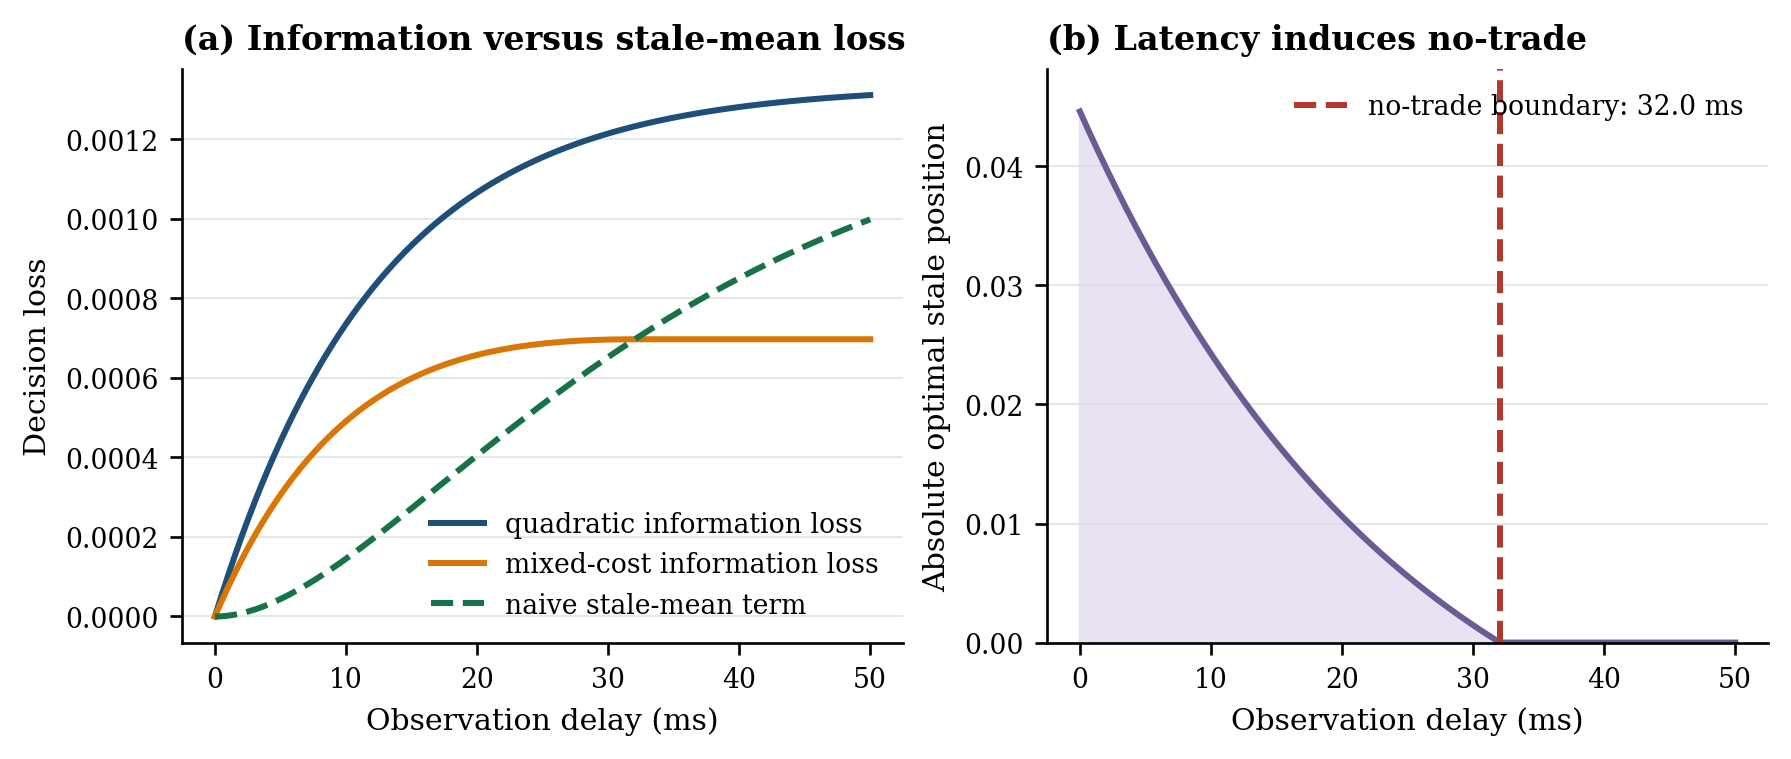
\includegraphics[width=\linewidth]{figures/04_latency_frontier.png}
\caption{Exact two-state latency frontier. Panel (a) separates quadratic
information loss, mixed-cost information loss, and the additional
quadratic loss from using an unpropagated stale mean. The objectives differ,
so the blue and orange curves are not one policy comparison. Panel (b)
shows the mixed-cost position shrinking to zero at the analytic boundary
\(\delta_{\rm stop}=32.0\) ms. The calculation uses the declared synthetic
parameters \(\kappa=20\), \(b=2\), \(h=0.05\), \(a=0.7\), and \(c=0.012\).}
\label{fig:latencyfrontier}
\end{figure}

\section{A joint certificate for forecasts, impact, and constraints}

\subsection{The adapted space and its causal adjoint}

Fix a finite horizon and an exogenous probability space with
filtration \((\mathcal G_t)_{0\le t\le T}\) satisfying the usual
conditions. Let
\(\mathsf H=L^2_{\mathrm{prog}}(\Omega\times[0,T];\R^d)\),
modulo equality almost everywhere, with
\(\ip{u}{v}=\E\int_0^T u_t^\top v_t\dd t\).
It is a closed Hilbert subspace of the ambient product \(L^2\) space.
A trading rate \(v\), from a deterministic initial position \(w_0\),
produces position
\(w_t=w_0+(Bv)_t\), where
\[
(Bv)_t=\int_0^t v_s\dd s .
\]
The operator is bounded, for example \(\norm B\le T\).
Its adjoint on this information class is
\begin{equation}\label{eq:causaladjoint}
(B^\ast z)_s=
\E\left[\int_s^T z_t\dd t\ \middle|\ \mathcal G_s\right],
\end{equation}
using a progressively measurable version. Indeed, Fubini and
conditional expectation give
\(\E\int z_t^\top\int_0^t v_s\dd s\dd t
=\E\int v_s^\top\E[\int_s^Tz_t\dd t\mid\mathcal G_s]\dd s\).
The required integrability follows from Cauchy--Schwarz.
The conditional expectation is essential: an unconditioned future
integral is the adjoint in a different, noncausal space.

Let \(\mathcal K\) be a bounded self-adjoint positive semidefinite
impact operator on \(\mathsf H\), let \(\gamma\ge0,\eta>0\), and
let \(\alpha\in\mathsf H\) be an exogenous expected-return-rate
process. The negative expected gain, up to terms independent of \(v\),
is
\begin{align}
\mathcal J(v)&=\tfrac12\ip{v}{Av}-\ip{f}{v}+\Psi(v),
\label{eq:pathobjective}\\
A&=2\eta I+\mathcal K+\gamma B^\ast B,\qquad
f=B^\ast(\alpha-\gamma w_0).\notag
\end{align}
Here \(\Psi\) can include a proportional turnover charge
\(c\,\E\int\norm{v_t}_1\dd t\) and the indicator of a common nonempty
closed convex feasible set. Pointwise rate bounds and the pathwise
mandate \(\int_0^T v_t\dd t=X\) are such constraints whenever jointly
feasible. The terminal integral is a bounded linear map into
\(L^2(\Omega)\), so its equality constraint is closed.
Every statement concerns rates; atomic endpoint blocks are outside
\(\mathsf H\).

For a scalar symmetric positive semidefinite kernel \(G(|t-s|)\),
with \(G\in L^1(0,T)\), its adapted energy operator is
\[
(\mathcal K v)_t=
\int_0^tG(t-s)v_s\dd s+
\E\left[\int_t^T G(s-t)v_s\dd s\ \middle|\ \mathcal G_t\right].
\]
It is the orthogonal compression of the symmetric kernel operator
to \(\mathsf H\), and is therefore self-adjoint and positive
semidefinite. Its quadratic form is the expected symmetric
transient-impact energy. These hypotheses give \(A\succeq2\eta I\);
no coercivity assertion about the transient kernel alone is needed.

\subsection{The joint residual and its exact affine form}

The next result uses the abstract form \eqref{eq:pathobjective}:
\(A,\widehat A\) are bounded self-adjoint operators on a common real
Hilbert space, bounded below by positive constants \(m,\widehat m\);
\(f,\widehat f\) belong to that space; and \(\Psi\) is a common proper
lower semicontinuous convex function.
The estimated objective replaces \(A,f\) by \(\widehat A,\widehat f\).
Both objectives have unique minimizers: an affine lower bound for
\(\Psi\) and positive quadratic curvature give coercivity, while
convex weak lower semicontinuity gives attainment.

\begin{theorem}[Joint model-and-optimization residual]\label{thm:jointresidual}
Let \(v^\ast\) minimize the true objective. For a feasible implemented
\(\widehat v\), suppose \(\widehat\xi\in\partial\Psi(\widehat v)\)
is supplied, and define
\[
\widehat s=\widehat A\widehat v-\widehat f+\widehat\xi,\qquad
r=(A-\widehat A)\widehat v-(f-\widehat f),\qquad s=r+\widehat s .
\]
Then
\begin{equation}\label{eq:jointresidual}
0\le\mathcal J(\widehat v)-\mathcal J(v^\ast)
\le\frac{\norm s^2}{2m},\qquad
\norm{\widehat v-v^\ast}\le\frac{\norm s}{m}.
\end{equation}
In particular, if
\(\norm{A-\widehat A}\le\epsilon_A\),
\(\norm{f-\widehat f}\le\epsilon_f\),
\(\norm{\widehat v}\le R\), and \(\norm{\widehat s}\le\tau\), then
the loss is at most
\[
\frac{(\epsilon_A R+\epsilon_f+\tau)^2}{2m}.
\]
An exact estimated optimizer admits \(\widehat s=0\).
\end{theorem}
\begin{proof}
The sum rule for a continuous differentiable quadratic and a proper
closed convex function gives
\(s=A\widehat v-f+\widehat\xi\in\partial\mathcal J(\widehat v)\).
Strong convexity gives, for every \(u\),
\[
\mathcal J(u)\ge\mathcal J(\widehat v)
 +\ip{s}{u-\widehat v}+\frac m2\norm{u-\widehat v}^2.
\]
Set \(u=v^\ast\) and complete the square to obtain the loss bound.
Strong monotonicity between \(s\) and
\(0\in\partial\mathcal J(v^\ast)\) gives
\(m\norm{\widehat v-v^\ast}^2
\le\ip{s}{\widehat v-v^\ast}\), proving the distance bound.
The triangle inequality proves the error-budget form. Fermat's rule
for the estimated objective supplies the zero residual at its minimizer.
\end{proof}

The estimate includes interactions between forecast and impact errors:
their residuals can reinforce or cancel. Adding separate forecast and
impact losses as if they were independent would generally discard that
interaction. For arbitrary convex constraints the inequality is the
appropriate statement; the exact quadratic equality requires an affine
class.

\begin{corollary}[Exact affine certificate and decision equivalence]
\label{cor:affineresidual}
Let \(\Psi\) be the indicator of a nonempty closed affine space
\(\mathcal M=v_0+V\), and let \(\widehat v\) be its exact estimated
optimizer. With orthogonal projection \(P_V\), put
\[
r_V=P_V[(A-\widehat A)\widehat v-(f-\widehat f)],\qquad
A_V=P_VA|_V .
\]
Then
\begin{equation}\label{eq:affineexact}
\widehat v-v^\ast=A_V^{-1}r_V,\qquad
\mathcal J(\widehat v)-\mathcal J(v^\ast)
=\tfrac12\ip{r_V}{A_V^{-1}r_V}.
\end{equation}
The two models produce the same implemented optimum if and only
if \(r_V=0\). Thus full identification of either primitive is not
necessary for decision equivalence on the declared affine class.
\end{corollary}
\begin{proof}
Stationarity gives
\(P_V(Av^\ast-f)=P_V(\widehat A\widehat v-\widehat f)=0\).
Subtract to obtain \(A_V(\widehat v-v^\ast)=r_V\).
The compressed operator is self-adjoint and bounded below by \(m\),
so it has a bounded inverse. Expansion around \(v^\ast\) kills the
linear term on \(V\), giving
\(\mathcal J(\widehat v)-\mathcal J(v^\ast)
=\ip{\widehat v-v^\ast}{A(\widehat v-v^\ast)}/2\).
Substitution proves the identity and the equivalence.
\end{proof}

For deterministic rates, \(f=\widehat f=0\), and fixed total mass,
the projection is onto zero-mass variations and the formula is the
execution-kernel residual. Retaining the signal gives the joint
forecast-and-execution version. On a finite common feature class,
the operators become matrices, and the subgradient residual is
an ordinary constrained optimization certificate. Coefficient-space
curvature also depends on the feature Gram matrix: redundant features
must be removed or quotiented before an invertible compressed matrix
can be claimed.
These conclusions require a common probability law for the exogenous
drivers and a common feasible class. A misspecified law of an
endogenous controlled book is not silently absorbed by changing
an impact matrix in this theorem.

\subsection{The forecast error seen through feasible trajectories}

Suppose only the forecast is misspecified: the operators, initial
position, and affine feasible class are common. Write
\(z=\alpha-\widehat\alpha\in\mathsf H\). The model residual then
contains only the causal adjoint of \(z\).

\begin{corollary}[Causally filtered forecast error]
\label{cor:filteredforecast}
In Corollary~\ref{cor:affineresidual}, assume
\(A=\widehat A\) and \(f-\widehat f=B^\ast z\). Define
\[
e=B^\ast z,\qquad
e_s=\E\left[\int_s^T(\alpha_t-\widehat\alpha_t)\dd t
                              \ \middle|\ \mathcal G_s\right].
\]
Then
\begin{align}
\mathcal J(\widehat v)-\mathcal J(v^\ast)
&=\tfrac12\ip{P_Ve}{A_V^{-1}P_Ve}\notag\\
&\le\frac{\norm{P_Ve}^2}{2m}
\le\frac{2T^2}{m\pi^2}\norm{\alpha-\widehat\alpha}^2.
\label{eq:filteredforecast}
\end{align}
The two forecasts induce the same rate, and hence the same position
trajectory from the common initial position, if and only if
\(P_Ve=0\). The final constant is sharp over the class with
\(A\succeq mI\).
\end{corollary}
\begin{proof}
The projected residual is \(r_V=-P_Ve\), so
\eqref{eq:affineexact} gives the identity. The inverse bound
\(A_V^{-1}\preceq m^{-1}I\) gives the first inequality.
For the second, the integration operator on \(\mathsf H\) has
\begin{equation}\label{eq:sharpvolterra}
\norm B=\norm{B^\ast}=2T/\pi.
\end{equation}
To see the upper bound, for each path put \(w=Bv\), so \(w(0)=0\).
Reflect \(w\) evenly about \(T\) onto \([0,2T]\); the reflected
function is zero at both endpoints. The Dirichlet Poincar\'e inequality
on that interval, obtained from its sine expansion, gives
\(\int_0^T|w|^2\le(2T/\pi)^2\int_0^T|v|^2\).
Average over paths. Equality is attained by the deterministic rate
\(v_t=u\cos(\pi t/(2T))\), with a fixed unit vector \(u\).
This rate is adapted to every filtration, so compression to
\(\mathsf H\) does not reduce the operator norm.
Now use \(\norm{P_VB^\ast z}\le\norm B\norm z\).
When \(V=\mathsf H\), \(A=mI\), and
\(z_t=u\sin(\pi t/(2T))\), every inequality in
\eqref{eq:filteredforecast} is an equality. This also proves
sharpness of its constant. Decision equivalence follows from
\eqref{eq:affineexact} and injectivity of rate integration.
\end{proof}

The error is measured after conditional remaining-horizon integration
and projection onto feasible directions. For a deterministic persistent
bias \(z_t=b\), \(e_s=b(T-s)\) and
\[
\frac{\norm e^2}{\norm z^2}=T^2/3
\quad(b\ne0),\qquad
\sup_{z\ne0}\frac{\norm{B^\ast z}^2}{\norm z^2}=4T^2/\pi^2.
\]
Thus constant bias is not a worst-case error at fixed \(L^2\) norm.
The maximizing error shape in the isotropic unconstrained example is
the sine profile in the proof. With other impact operators or feasible
directions, the worst shape is determined by
\(A_V^{-1/2}P_VB^\ast\), rather than by persistence alone.
For the trading objective \eqref{eq:pathobjective}, taking
\(m=2\eta\) gives the bound
\(T^2\norm{\alpha-\widehat\alpha}^2/(\eta\pi^2)\).

Projection can suppress error components on a restricted feasible
class, precisely when \(P_VB^\ast z=0\). In the full adapted space
\(V=\mathsf H\), there is no nonzero adapted \(z\) with
\(B^\ast z=0\). Indeed, write
\(B^\ast z=M-\int_0^\cdot z_t\dd t\), where
\(M_s=\E[\int_0^Tz_t\dd t\mid\mathcal G_s]\).
If this process vanishes almost everywhere, its c\`adl\`ag version
vanishes on \([0,T)\), and at \(T\) the same identity is zero by
definition. The martingale \(M\) is then a continuous finite-variation
process, hence constant, forcing \(z=0\) almost everywhere.

\subsection{Information loss and model loss are orthogonal on affine classes}

Let \(\mathcal M_G\subset\mathcal M_F\) be nonempty closed affine
subspaces of a common Hilbert space, representing two information
classes with the same underlying quadratic objective
\(\mathcal J_0(v)=\ip{v}{Av}/2-\ip{f}{v}\), \(A\succeq mI\).
Let \(v_G^\ast,v_F^\ast\) be their true optimizers. Define
\(\norm u_A^2=\ip{u}{Au}\).

\begin{theorem}[Information projection and residual decomposition]
\label{thm:informationprojection}
For every \(\widehat v\in\mathcal M_G\),
\begin{equation}\label{eq:informationprojection}
\mathcal J_0(\widehat v)-\mathcal J_0(v_F^\ast)
=\tfrac12\norm{v_G^\ast-v_F^\ast}_A^2
 +\tfrac12\norm{\widehat v-v_G^\ast}_A^2.
\end{equation}
If \(\widehat v\) is the exact estimated optimizer on \(\mathcal M_G\),
the second term equals
\(\ip{r_G}{A_G^{-1}r_G}/2\), with the projection and compression
defined as in Corollary~\ref{cor:affineresidual} for its direction space.
\end{theorem}
\begin{proof}
Let \(V_G\subset V_F\) be the direction spaces.
Stationarity of both optima implies
\(\ip{A(v_G^\ast-v_F^\ast)}{z}=0\) for every \(z\in V_G\).
Take \(z=\widehat v-v_G^\ast\).
Expansion around \(v_F^\ast\) first gives
\(\mathcal J_0(\widehat v)-\mathcal J_0(v_F^\ast)
=\norm{\widehat v-v_F^\ast}_A^2/2\).
The vanished cross term splits this square into the two displayed
energies. The residual form follows from
Corollary~\ref{cor:affineresidual}.
\end{proof}

The first term is the cost of the restricted information class for
this objective, and remains with a perfectly estimated model.
The second is the cost of the implemented rule within that class.
This is a Hilbert projection statement, not a mutual-information
formula. With general convex constraints, value differences still
separate algebraically, but these orthogonal energy equalities
need not hold. Both benchmarks must evaluate the same objective;
enlarging a price filtration can change an economic return model,
which must then be specified separately.

\begin{example}[A two-date information and model decomposition]
\label{ex:informationtree}
Let \(Z=\pm1\) with equal probability. At two dates choose rates
\((v_0,v_1)\) with \(v_0+v_1=1\) in every scenario, and minimize
\[
\mathcal J_0(v)=
\E\big[\tfrac12(v_0^2+v_1^2)-Zv_0\big].
\]
The richer class sees \(Z\) before the first rate. Its optimum is
\((1,0)\) when \(Z=1\), and \((0,1)\) when \(Z=-1\), with value
zero. In the restricted class, \(v_0\) is chosen before \(Z\) is
revealed; completion then fixes \(v_1\). Its optimum is the constant
\((1/2,1/2)\), with value \(1/4\).
Replacing the first-date signal \(Z\) by \(Z+1/5\) in the restricted
optimization gives the implemented rates \((3/5,2/5)\).
Their true cost is \(13/50\), and
\[
\underbrace{13/50}_{\text{total loss}}
=\underbrace{1/4}_{\text{information loss}}
 +\underbrace{1/100}_{\text{model loss}}.
\]
Both energy terms are exact rational quantities. Better estimation
within the restricted class can remove the second term, but not
the first.
\end{example}

\section{Causal trading of a mean-reverting target}

\subsection{Admissible tracking and an exact verification identity}

Let \(x_t\) be a stationary OU target on the real time line:
\[
\dd x_t=-\rho x_t\dd t+\sqrt{2\rho v}\dd B_t,\qquad \rho,v>0.
\]
Its filtration is the completed natural filtration of its observed
history. A trading position \(w\) is adapted, absolutely continuous with
\(\dot w_t=u_t\), and jointly stationary with \(x\) and \(u\).
Admissibility requires \(\E(w_t^2+u_t^2)<\infty\).
For \(\eta,\kappa>0\), minimize
\[
J(w)=\E\big[\eta u_t^2+\eta\kappa^2(w_t-x_t)^2\big].
\]
The earlier risk notation is recovered from
\(\kappa^2=\gamma\sigma^2/(2\eta)\).
The expectation is a stationary average cost per unit time.

\begin{theorem}[Causal optimum and exact excess cost]\label{thm:causal}
Set \(\theta=\kappa/(\kappa+\rho)\).
The optimal stationary adapted policy is
\begin{equation}\label{eq:causalpolicy}
u_t=\kappa(\theta x_t-w_t),\qquad
w_t=\kappa\theta\int_0^\infty e^{-\kappa s}x_{t-s}\dd s .
\end{equation}
Its minimum cost is
\begin{equation}\label{eq:causalvalue}
J^\ast=\eta\kappa^2v(1-\theta^2).
\end{equation}
Every admissible stationary rule satisfies the exact identity
\begin{equation}\label{eq:trackingregret}
J(w)-J^\ast
=\eta\,\E\!\left[\big(u_t+\kappa(w_t-\theta x_t)\big)^2\right].
\end{equation}
The optimal position is unique among admissible stationary solutions,
up to equality almost surely.
\end{theorem}
\begin{proof}
Define the quadratic relative value function
\[
\mathcal V(w,x)=
\eta\kappa w^2-2\eta\kappa\theta wx
 +\frac{\eta\kappa^2}{2\rho}(1-\theta^2)x^2.
\]
For a control \(u\), its generator is
\(\mathcal L^u\mathcal V
=u\mathcal V_w-\rho x\mathcal V_x+\rho v\mathcal V_{xx}\).
Direct expansion, using \(\rho\theta=\kappa(1-\theta)\), gives
\begin{equation}\label{eq:hjbsquare}
\eta u^2+\eta\kappa^2(w-x)^2+\mathcal L^u\mathcal V
=\eta\kappa^2v(1-\theta^2)
 +\eta\big[u+\kappa(w-\theta x)\big]^2.
\end{equation}
For an admissible stationary control, Ito's formula on a finite time
interval and stationarity give \(\E\mathcal L^u\mathcal V=0\).
The stochastic integral is square integrable because its integrand is
linear in \(w,x\), which have finite second moments. All drift terms are
integrable by Cauchy--Schwarz. Averaging \eqref{eq:hjbsquare} proves
\eqref{eq:trackingregret}.

The stable causal convolution in \eqref{eq:causalpolicy} is adapted,
has finite second moments and finite trading-rate cost, and makes the
square zero. It therefore attains \eqref{eq:causalvalue}.
Equality for any other optimizer requires the same linear differential
equation. For two solutions, their difference at \(t\) equals
\(e^{-\kappa(t-s)}\) times its value at any earlier \(s\).
Both solutions have uniformly bounded second moments on the real time
line. Letting \(s\to-\infty\) forces the difference at \(t\) to be
zero in \(L^2\). Thus the stationary optimizer is unique.
\end{proof}

The aim is \(\theta x_t\), whereas the position is the lagged
convolution in \eqref{eq:causalpolicy}. Indeed
\[
\kappa\int_0^\infty e^{-\kappa s}\E_t[x_{t+s}]\dd s=\theta x_t.
\]
This conditional future average defines the aim, not the position.
The policy is the scalar continuous-time analogue of the aim-portfolio
structure in \citet{GarleanuPedersen2013}.

\begin{corollary}[Using a wrong tracking rule]\label{cor:wrongtracking}
Consider any stable linear rule
\(\dot w_t=-\alpha w_t+\beta x_t\), with \(\alpha>0\).
Then
\[
J(w)-J^\ast=
\eta\,\E\!\left[\big((\kappa-\alpha)w_t+
                 (\beta-\kappa\theta)x_t\big)^2\right],
\]
where
\[
\E[w_tx_t]=\frac{\beta v}{\alpha+\rho},\qquad
\E[w_t^2]=\frac{\beta^2v}{\alpha(\alpha+\rho)}.
\]
Small errors in \(\alpha,\beta\) around
\((\kappa,\kappa\theta)\) cause second-order excess cost on parameter
sets bounded away from instability.
\end{corollary}
\begin{proof}
Substitute the rule in \eqref{eq:trackingregret}. The stationary moment
equations for \(wx\) and \(w^2\) give the two covariances. These moments
remain bounded on compact stable parameter sets, so the quadratic
residual has the stated rate.
\end{proof}

\begin{corollary}[Misspecified persistence and friction]
\label{cor:wrongprimitives}
Keep the true stationary target law, \(\eta,\kappa,\rho,v>0\), and
\(\theta=\kappa/(\kappa+\rho)\).
\begin{enumerate}
\item If only target persistence is misspecified, let
\(\widehat\rho>0\),
\(\widehat\theta=\kappa/(\kappa+\widehat\rho)\), and use
\(\dot w_t=\kappa(\widehat\theta x_t-w_t)\). Then
\begin{equation}\label{eq:wrongpersistence}
J(w)-J^\ast=\eta\kappa^2v(\widehat\theta-\theta)^2,
\qquad
\frac{J(w)-J^\ast}{J^\ast}
=\frac{(\widehat\theta-\theta)^2}{1-\theta^2}.
\end{equation}
\item If the target's decay rate is correct but the trading rate is
\(\widehat\kappa>0\), let
\(\widehat\theta=\widehat\kappa/(\widehat\kappa+\rho)\) and use
\(\dot w_t=\widehat\kappa(\widehat\theta x_t-w_t)\). Then
\begin{align}
J(w)-J^\ast=\eta v\big[&
 (\kappa-\widehat\kappa)^2\widehat\theta^3
 +(\widehat\kappa\widehat\theta-\kappa\theta)^2\notag\\
 &+2(\kappa-\widehat\kappa)
       (\widehat\kappa\widehat\theta-\kappa\theta)
          \widehat\theta^2\big].\label{eq:wrongfriction}
\end{align}
\end{enumerate}
In the fixed-risk specification
\(\kappa^2=\gamma\sigma^2/(2\eta)\), an estimated friction
\(\widehat\eta>0\) corresponds to
\(\widehat\kappa=\sqrt{\gamma\sigma^2/(2\widehat\eta)}\).
All losses above are evaluated using the true objective coefficients.
\end{corollary}
\begin{proof}
Apply Corollary~\ref{cor:wrongtracking}. In the first case,
\((\alpha,\beta)=(\kappa,\kappa\widehat\theta)\), so the coefficient
of \(w\) in the square vanishes and \(\E x_t^2=v\).
In the second case,
\((\alpha,\beta)=(\widehat\kappa,\widehat\kappa\widehat\theta)\),
and the stationary moments are
\(\E[w_tx_t]=v\widehat\theta^2\) and
\(\E[w_t^2]=v\widehat\theta^3\). Expanding the residual square
gives \eqref{eq:wrongfriction}. The nonnegativity of this expression
follows from that square, even when its cross term is negative.
\end{proof}

For equal errors of magnitude \(d\), with \(0<d<\rho\), the ratio
of the excess cost from \(\widehat\rho=\rho-d\) to that from
\(\widehat\rho=\rho+d\) is exactly
\[
\left(\frac{\kappa+\rho+d}{\kappa+\rho-d}\right)^2>1.
\]
Underestimating mean reversion is more costly in this comparison.
Locally, with \(d=\widehat\rho-\rho\),
\[
J(w)-J^\ast=\eta v\theta^4d^2+O(|d|^3),
\qquad \frac{\dd\theta}{\dd\rho}=-\theta^2/\kappa.
\]
For random estimates independent of the subsequently evaluated
stationary target, supported in a fixed compact positive parameter
interval, this gives
\[
\E[J(w)-J^\ast]
=\eta v\theta^4\E(\widehat\rho-\rho)^2
  +O\big(\E|\widehat\rho-\rho|^3\big).
\]
The leading term uses estimation MSE, including squared bias;
variance alone is sufficient only for an unbiased estimate. These
formulas evaluate fixed stationary policies, or an independent mixture
of them, and do not assert the same result for a continuously updated
estimate coupled to the live target.

\subsection{Covariance, correlation, and the cost of causality}

\begin{proposition}[Three distinct transfer quantities]\label{prop:transfer}
For the optimal causal rule,
\[
\frac{\Cov(w_t,x_t)}v=\theta^2,\qquad
\frac{\Var(w_t)}v=\theta^3,\qquad
\Corr(w_t,x_t)=\sqrt{\theta}.
\]
If future target values are also available, the minimum tracking cost
is \(J_s=\eta\kappa^2v(1-\theta)\). Its two-sided smoothing filter has
transfer function
\[
H_s(\omega)=\frac{\kappa^2}{\kappa^2+\omega^2}
\]
and normalized covariance \(\Cov(w_t^s,x_t)/v=\theta\).
Consequently
\begin{equation}\label{eq:causalitycost}
J^\ast-J_s=\eta\kappa^2v\,\theta(1-\theta),\qquad
\frac{J^\ast-J_s}{J^\ast}=\frac{\theta}{1+\theta}.
\end{equation}
\end{proposition}
\begin{proof}
For the causal policy, stationarity gives
\[
0=-(\kappa+\rho)\E[wx]+\kappa\theta v,\qquad
0=-2\kappa\E[w^2]+2\kappa\theta\E[wx].
\]
Thus \(\E[wx]=v\theta^2\) and \(\E[w^2]=v\theta^3\);
division by the standard deviations gives the correlation.

For the unconstrained smoother, the spectral density of the target is
\(S_x(\omega)=2\rho v/(\rho^2+\omega^2)\).
Completing the square frequency by frequency in the tracking criterion
gives \(H_s\). Equivalently, convolution with
\(\kappa e^{-\kappa|s|}/2\) solves the unconstrained Euler equation;
stationarity and integration by parts give, for every finite-cost
jointly stationary competitor,
\[
J(w)-J(w^s)=
\eta\E\big[(u_t-u_t^s)^2+\kappa^2(w_t-w_t^s)^2\big].
\]
The cross term vanishes because
\(\dot u_t^s=\kappa^2(w_t^s-x_t)\).
This verifies the minimizer beyond the class of linear filters.
Its impulse response has negative-time support, so it
is not implementable with the observed-history filtration.
The integral
\[
\int_{-\infty}^{\infty}
\frac{\dd\omega}{2\pi(\kappa^2+\omega^2)(\rho^2+\omega^2)}
=\frac{1}{2\kappa\rho(\kappa+\rho)}
\]
gives \(\E[w^sx]=v\theta\).
At the minimizing frequency response the cost integrand is
\(\eta\kappa^2(1-H_s)S_x\), hence \(J_s=\eta\kappa^2v(1-\theta)\).
Subtracting from \eqref{eq:causalvalue} proves \eqref{eq:causalitycost}.
\end{proof}

\begin{center}
\begin{tabular}{@{}rrrrr@{}}
\toprule
\(\rho/\kappa\)&Causal covariance/\(v\)&Correlation&
\(J^\ast/(\eta\kappa^2v)\)&Causality share of \(J^\ast\)\\
\midrule
1&\(1/4\)&\(1/\sqrt2\)&\(3/4\)&\(1/3\)\\
2&\(1/9\)&\(1/\sqrt3\)&\(8/9\)&\(1/4\)\\
10&\(1/121\)&\(1/\sqrt{11}\)&\(120/121\)&\(1/12\)\\
\bottomrule
\end{tabular}
\end{center}

The normalization matters. A target decaying twice as fast as the
trading rate produces normalized covariance \(1/9\), Pearson
correlation \(1/\sqrt3\), and a causality increment equal to one
quarter of the optimal causal tracking cost. None is a direct fraction
of a strategy's profit or Sharpe ratio. Halving \(\eta\) at fixed
\(\gamma\sigma^2\) increases \(\kappa\) by \(\sqrt2\); other comparative
statics must account for the resulting changes in both scale and
normalization.

Figure~\ref{fig:causaltracking} contrasts an illustrative causal path with
the exact transfer quantities of Proposition~\ref{prop:transfer}.

\begin{figure}[tbp]
\centering
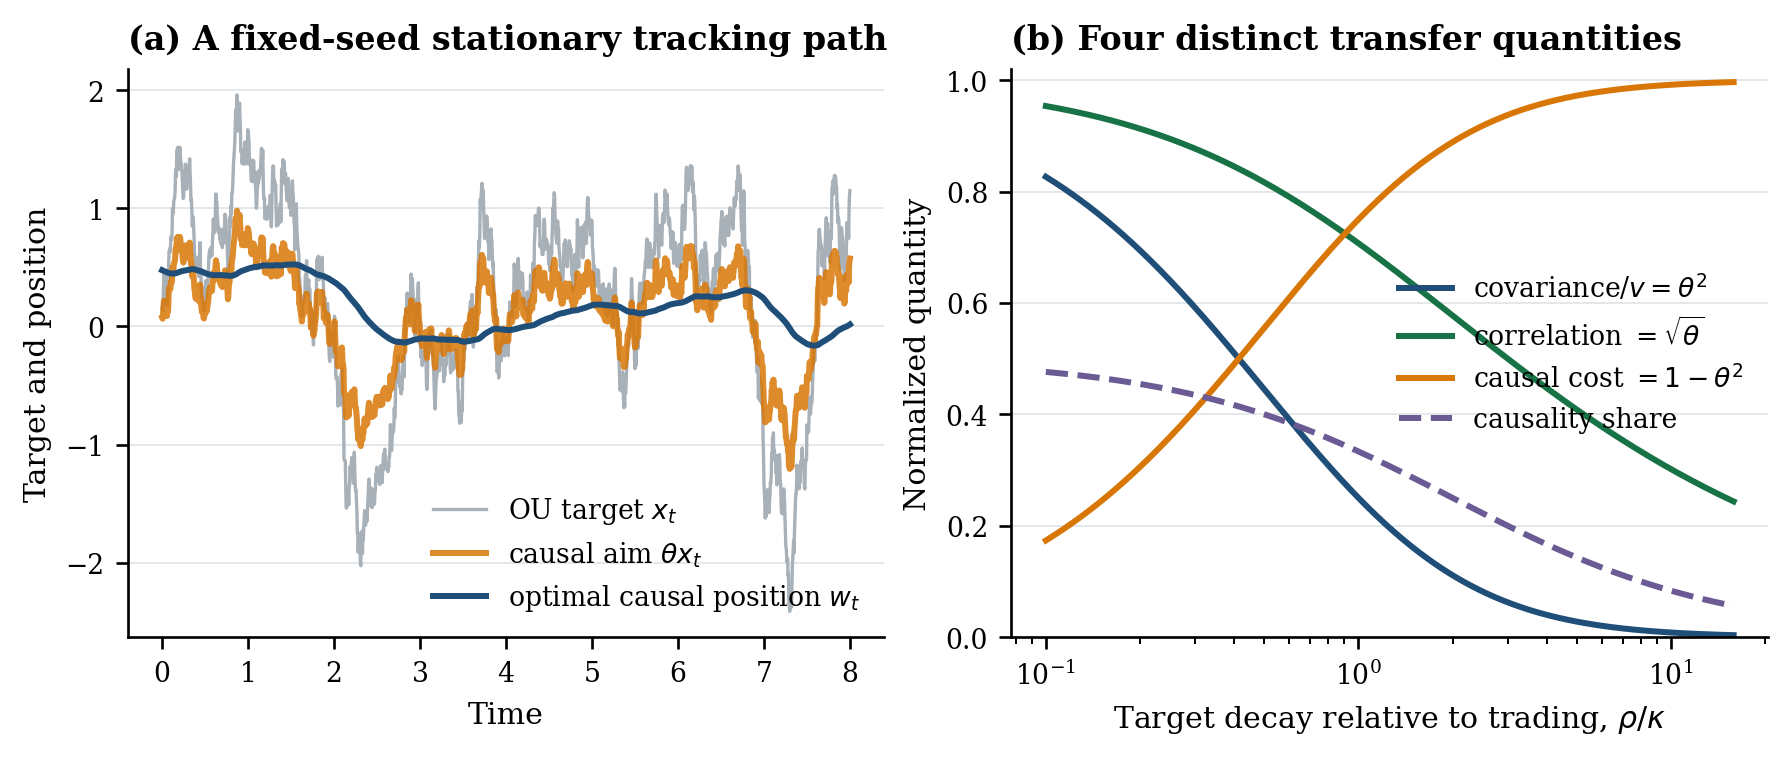
\includegraphics[width=\linewidth]{figures/05_causal_tracking.png}
\caption{Causal tracking of a stationary mean-reverting target. Panel (a)
shows a fixed-seed discretization with \(\rho=\kappa=v=1\), after an
eight-unit burn-in: the aim is \(\theta x_t\), whereas the implementable
position is its lagged causal filter. Panel (b) gives the exact normalized
covariance \(\theta^2\), correlation \(\sqrt\theta\), causal cost
\(1-\theta^2\), and causality share \(\theta/(1+\theta)\) as functions of
\(\rho/\kappa\), where \(\theta=(1+\rho/\kappa)^{-1}\). The sample path is
illustrative; the four transfer curves are analytic.}
\label{fig:causaltracking}
\end{figure}

\section{Information and logarithmic growth}

An information bound requires an explicit portfolio opportunity set.
It does not automatically cap a quadratic utility measured in
different units.

\begin{theorem}[Portfolio information ceiling]\label{thm:information}
Let the gross-return vector \(R\in[\underline r,\overline r]^d\), with
\(0<\underline r\le\overline r<\infty\), and let admissible portfolios
be the simplex \(\Delta_d=\{b\ge0:\sum_i b_i=1\}\).
For a signal \(Y\) on a standard Borel space, the improvement in
optimal one-period expected
logarithmic growth satisfies
\[
0\le
\E_Y\max_{b\in\Delta_d}\E[\log(b^\top R)\mid Y]
 -\max_{b\in\Delta_d}\E\log(b^\top R)
\le I(R;Y).
\]
The market and feasible portfolio set are the same with and without
the signal.
\end{theorem}
\begin{proof}
Let \(b_0\) maximize the unconditional objective; compactness and the
bounded positive returns ensure existence. Its directional optimality
condition toward any \(b\in\Delta_d\) gives
\[
\E\frac{b^\top R}{b_0^\top R}\le1.
\]
For a conditional law \(P_y\) and unconditional law \(P\), the
variational relative-entropy inequality implies
\[
\E_{P_y}\log\frac{b^\top R}{b_0^\top R}
\le\KL(P_y\Vert P)
 +\log\E_P\frac{b^\top R}{b_0^\top R}
\le\KL(P_y\Vert P).
\]
If the relative entropy is infinite the assertion is immediate.
Apply the inequality to a conditional maximizing portfolio and
average over \(Y\). The expectation of the baseline conditional
log return is its unconditional value. Ignoring \(Y\) gives the
lower bound.
\end{proof}

This is the classical log-optimal information comparison
\citep{Kelly1956,CoverThomas2006}, under convenient bounded-return
assumptions. In the separate finite horse-race model, with positive
outcome probabilities and outcome-specific payoffs, the optimal
conditional betting proportions give equality with mutual information.
The simplex and positivity assumptions cannot be dropped while
retaining an unrestricted assertion about arbitrary actions and
arbitrary logarithmic rewards.

\section{Scope and implications}

The loss metric is determined jointly by the objective and the feasible
set. A quadratic objective gives an exact weighted MSE. Positive
curvature preserves a quadratic upper bound even with proportional
costs and convex constraints. Without curvature, a threshold decision
admits a uniform linear-in-error bound. Margin assumptions give sharper
average rates, but a global MSE budget permits errors to concentrate at
decision boundaries. The fixed-law lower construction shows that this
distinction changes the best uniform exponent. When diameter and
curvature coexist, their sharp combined envelope has a quadratic branch
and a linear branch; the actual loss can be strictly smaller.
For scalar interval uncertainty, the conjugate-secant position
minimizes worst-case loss exactly without requiring curvature.
The interval radius is quadratic for quadratic friction, linear
at a proportional-cost threshold, and zero within a common
no-trade region. Queue depletion realizes the endpoint means,
so these minimax lower bounds also hold in a marked book model.

The adapted-space certificate combines forecast and impact errors
before squaring the residual, and keeps the common convex constraints
explicit. Its affine form identifies exactly the model discrepancies
that leave the optimal decision unchanged. With nested affine
information classes, loss separates into an irreducible information
energy and an additional implementation energy. These are conditional
statements about a fixed quadratic objective and exogenous law.
With known impact, causal integration and projection specify the
forecast-error metric exactly. Constant bias does not maximize that
metric in general. In the stationary tracking specialization, wrong
persistence and wrong friction have explicit excess costs, and the
local expected persistence loss depends on estimation MSE.

The order-book certificate retains event timing, price marks, hidden-state
inference, and state reduction. The event filter computes a posterior
under a declared parameter model; it does not identify those parameters
from data. Its perturbation bound can deteriorate on rare histories.
The coarse-state certificate includes both transition-rate and
price-compensator residuals, because transition lumpability alone
does not preserve marked price changes. The additive forecast's
three horizon coefficients are individually sharp. Positive
likelihood and future-increment enclosures can be substantially
more informative than a succession of norm bounds. Their validity
requires a positive history-likelihood lower bound, rigorous
arithmetic enclosures, and an uncertainty set containing the true
primitives. Their interval minimax claim applies to that interval,
which can enlarge a correlated parameter family.
A price-specific feature can preserve every conditional mean
without preserving the full transition law. This conclusion
requires the stated common friction and price compensator; a
state-dependent risk charge or fill objective can need additional
observables. The information decomposition also separates
unobserved current-state variation from model or implementation
error. In the delayed-feed model the former is generally linear
in small latency, even when the latter has a quadratic forecast
loss. The stationary latency frontier and its no-trade threshold
concern the specified observation experiment, with no additional
informative events between snapshots.
The OU result uses a fully observed, exogenous, stationary scalar target
and excludes terminal constraints and feedback of trading into the
target. Its excess-cost identity evaluates tracking rules within that
model. Extending these certificates to calibrated venue-specific books,
nonstationary latent processes, and endogenous impact requires
additional assumptions and analysis.

The accompanying checks verify exact formulas against independent
optimization, matrix-exponential, covariance, and finite-tree adjoint
calculations. Twenty-four random affine and mixed-constraint instances
check the joint residual; the largest affine-identity discrepancy is
below \(10^{-15}\). Exact rational calculations reproduce
Example~\ref{ex:informationtree}; numerical integrations recover the
sharp threshold exponents for \(\alpha=1/2,1,2\).
Additional checks verify the curvature--diameter envelope in 192
independent scalar optimizations, with rational examples attaining both
branches. Quadrature and a singular-value computation verify the sharp
causal integration constant. Ninety-six independent stationary
Lyapunov calculations check the persistence and friction formulas,
with maximum discrepancy below \(8\times10^{-15}\).
The event filter is independently compared with its normalized
nonlinear ODE, and the aggregation identity with matrix-exponential
quadrature. Example~\ref{ex:completebook} checks the complete transfer
from an observed event history through a reduced model to an
inexact position decision. Timing and state-reduction counterexamples
show why the declared observation and state variables matter.
The additional interval calculations use rational arithmetic to
enclose exponentials, future-price integrals, and normalized
forecasts. Independent optimization checks the minimax rule for
40 mixed-friction cases and three nonquadratic frictions;
exact examples attain its quadratic and threshold radii.
These computations distinguish numerical comparisons from the
analytic inequalities and outward rounding that certify a whole
uncertainty box.
These are synthetic verification exercises, not a comparison of neural
architectures or a backtest of market predictability.

\bibliographystyle{plainnat}
\bibliography{references}
\end{document}
